\subsection{Attempted rigging of Big Rock Candy Mountain alternative}

\margininbox{Big Rock traverse}{
     \begin{itemize}
    \item Jonathon Hardman
    \item Dave Wilson
    \end{itemize}}{\explo}

Dave and Jon set off for to try and rig to the window seen across
\passage{Big Rock Candy Mountain} the previous year. Attempting to start
from the top, Dave bolted leftwards from the top, slowly, slippily, and
still in the draught from the approach passage, but after a long time
spent placing only 6 bolts, had only reached 1/3 of the way down the
initial slope, getting into increasingly poor rock as he went.

Giving that up as a lost cause, D and J both descended \passage{Big Rock
Candy Mountain} to have a look from lower down. It became rapidly clear
that that would have been the right thing to do in the first place,
with, it seemed, only a few bolts needed to reach and then protect a
ledge route around to the bottom of the window. It also became clear
that the window wasn't a window at all, but a seemingly complete
parallel shaft, only divided from the bottom of \passage{Big Rock Candy
Mountain} by a $\approx$ 10-15 m high wall at the bottom, with no
visible division any higher up -- the `window' seen had been an illusion
caused by looking across from high up \passage{Big Rock Candy Mountain},
where an intervening overhang on the right hand wall had played the part
of the top of the window. It wasn't obvious how far down any parallel
shaft might go beyond the wall, since all that could really be seen from
any suitably high vantage points was blackness, but it did seem that the
parallel shaft was a good size in terms of diameter, maybe larger than
\passage{Big Rock Candy Mountain} itself.

On arrival at the bottom, the dividing wall was examined from below, but
no easy climbing routes were seen. A clutch of crabs and hangers were
retrieved from between the cobbles near the base of the rope, presumably
dropped by someone in a previous year, but still in very good condition,
so the day had not been entirely wasted.

\name{Dave Wilson}

\begin{pagefigure}
\checkoddpage \ifoddpage \forcerectofloat \else \forceversofloat \fi
   \centering
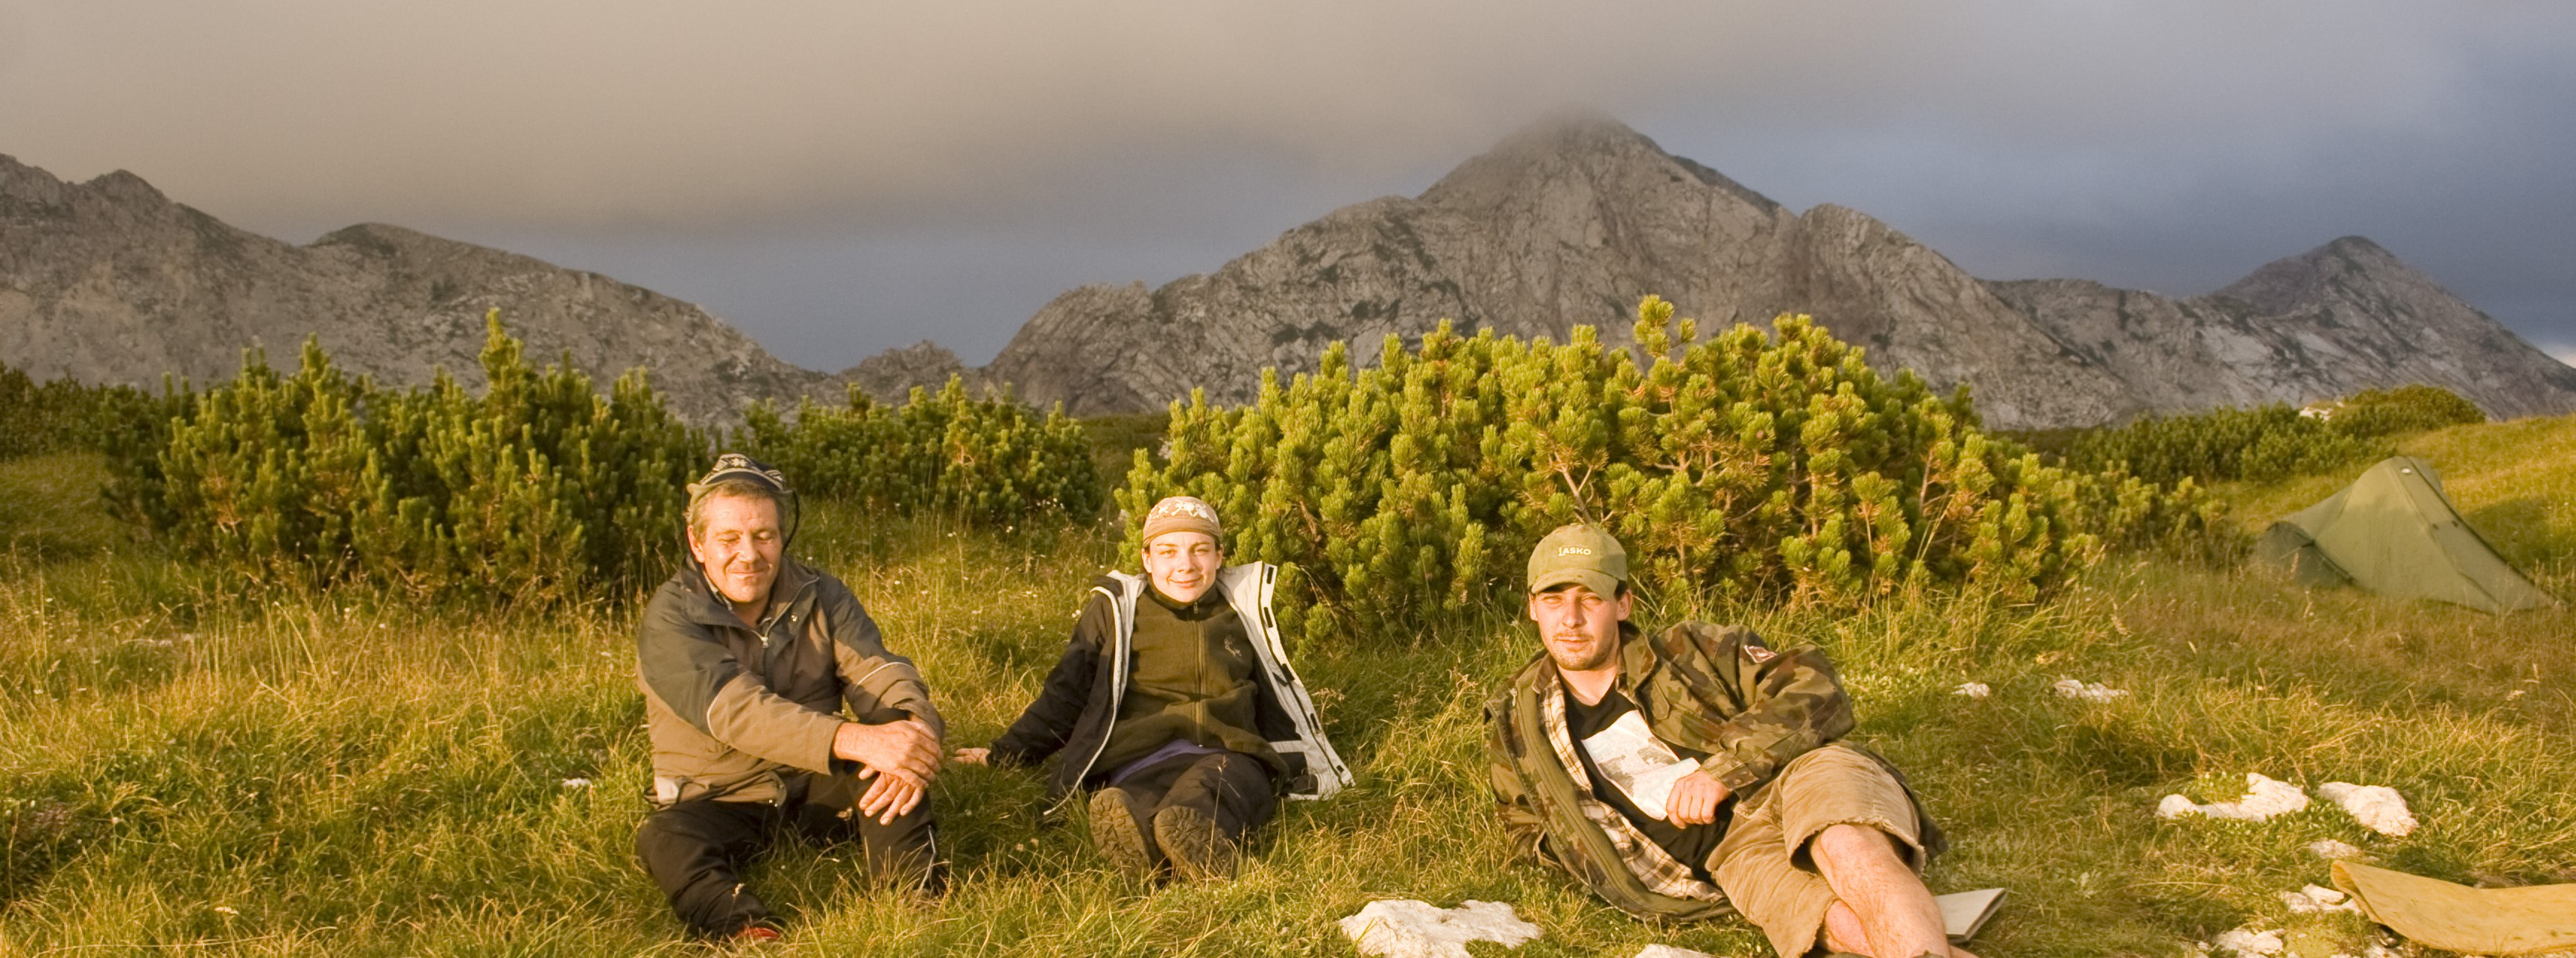
\includegraphics[width = \textwidth]{2011/winter_journey/2011-08-03-18.18.52-Jana Carga-Canon 350D--orig.jpg}
\caption{Gloomy clouds above \passage[mountain]{Skrbina} in the background while Kos, Jana and Izi appreciate the evening lighting in the foreground. \pic{Jana Čarga}} \label{gloom surface}
\end{pagefigure}


\newpage

\section{Dream 2 and Penguin's Egg}

\begin{marginfigure}
\checkoddpage \ifoddpage \forcerectofloat \else \forceversofloat \fi
\centering
 \frame{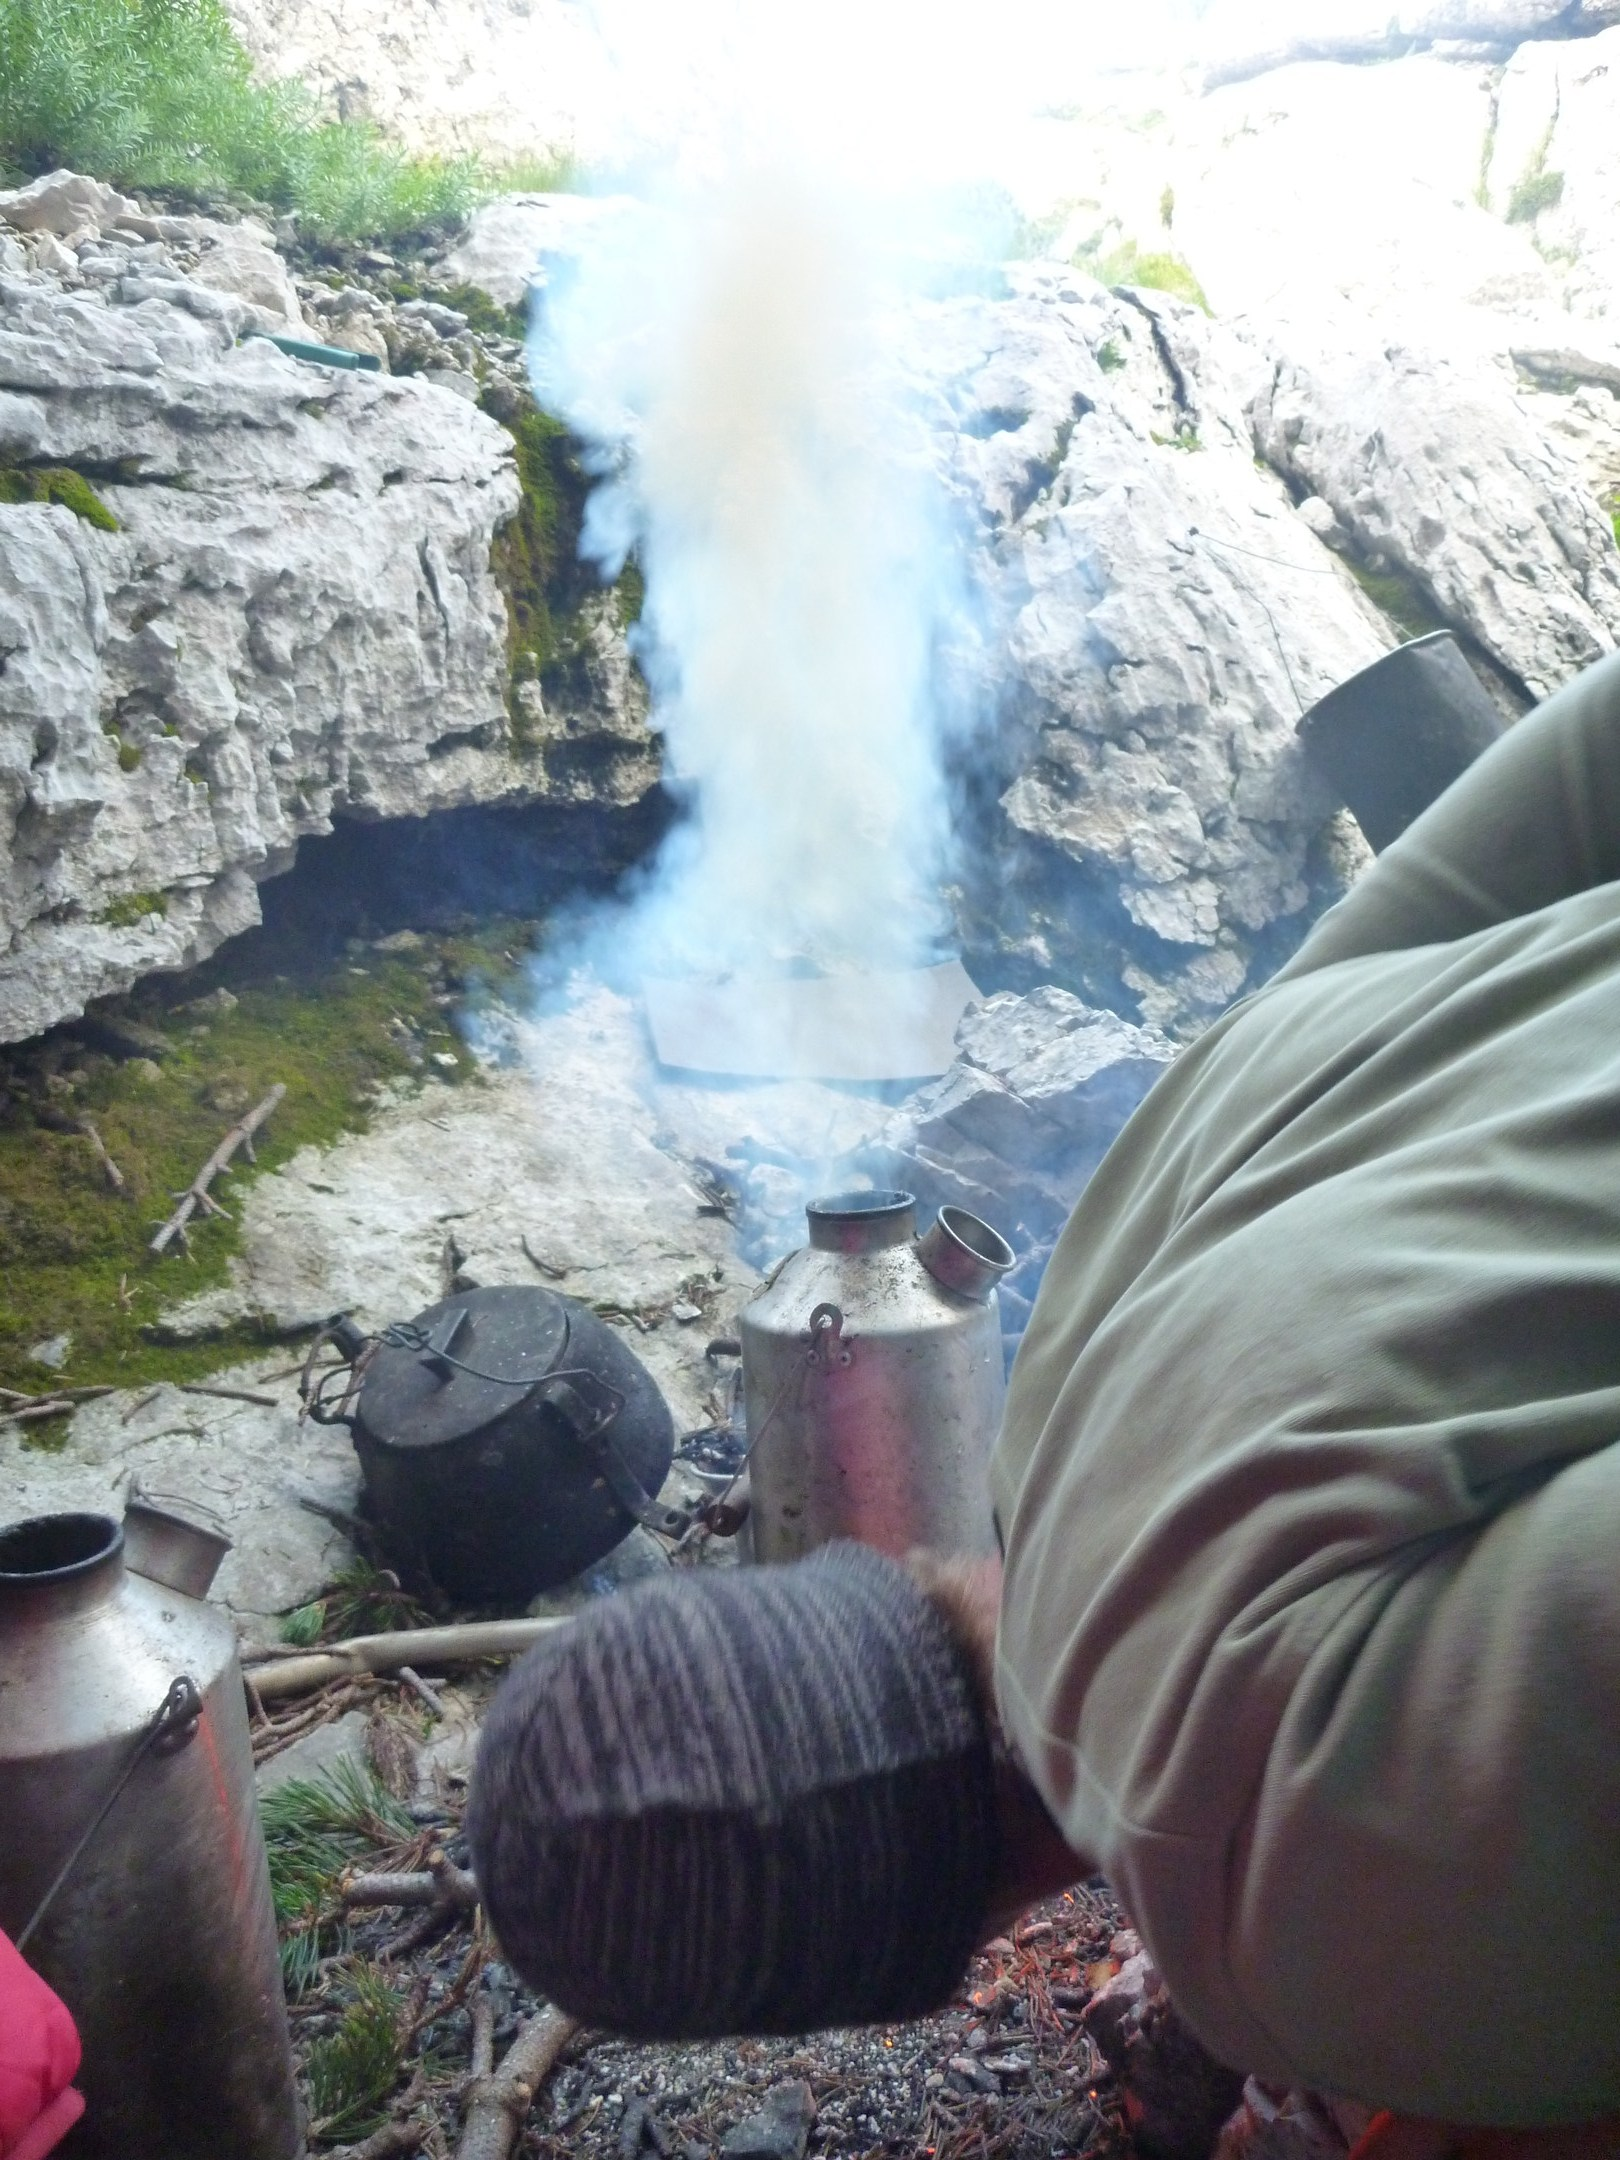
\includegraphics[width=\linewidth]{2011/winter_journey/2011-07-31-18.51.00-Grega-Panasonc DMC-FT2-066--orig.jpg}} 
 \caption{The Kelly Kettle churning out heat---and smoke---to boil water. \pic{Grega Maffi}}
 \label{kelly kettle smoke}
\end{marginfigure}

Morning. The weather was glorious: the sun was shining, and the sky more
blue than white---both rarities on this expedition. I knew there was
heavy rain forecast for the next few days, but for now, I sat on the
outcrop of limestone outside my tent, relishing the warmth of the sun's
rays on my cheeks.

Soon my need for my morning cup of tea became too great to ignore and I
ambled to the bivi, the shakehole that I'd already come to love and see
as home in a scant three weeks. This early in the morning, the bivi was
still relatively quiet as the masses snoozed in their tents, though
Tetley and Dan already had the volcano kettle going---perfect.

Brew in hand, I settled myself onto a `McGowan'\sidenote{sofas made of dwarf pine needles wrapped in tarp material} as
talk naturally turned to people's plans for the day.

``Samo's in a pretty bad shape, but I think I've managed to persuade him
to go down with me,'' said Tetley. They'd made plans to push
\passage{Daydreamers}, an active cascade series at the very bottom of
\passage{Vrtnarija}, but Samo had been a touch too liberal with the vino
the night before. ``I messed up last night,'' he continued, frustrated.
``All I had to say to him was `Be Ready', before I went to bed\ldots{}''

Sure enough, it wasn't long before Samo staggered into the \passage{Bivi}, looking
like he'd seen better days.

``Maybe we could go tomorrow instead. I'll be ready then,'' Samo
suggested.

``Nah, I want to go caving today\ldots{}''

Dan and I looked on in amusement. However, when a couple of mugs of tea
did little to alleviate his hangover, it soon became clear that Samo
wasn't in fit enough state to go pushing at -850 m in the next few
hours.

``Maybe\ldots{}'' Tetley began, eyes taking on that characteristic
gleam. Uh oh; I brace myself. Anyone who knows Tetley knows about him
and his `plans'. I could practically smell one forming in his mind.
``\ldots{}maybe I could go down with Clare today, push
\passage{Daydreamers}, then you and Karin can come down together tomorrow
to meet us at camp, and we can swap partners? Of course, I haven't even
discussed any of this with Clare yet\ldots{}''

``Yeah, you haven't!'' I nod, eyebrows raised.

\begin{marginfigure}
\checkoddpage \ifoddpage \forcerectofloat \else \forceversofloat \fi
\centering
 \frame{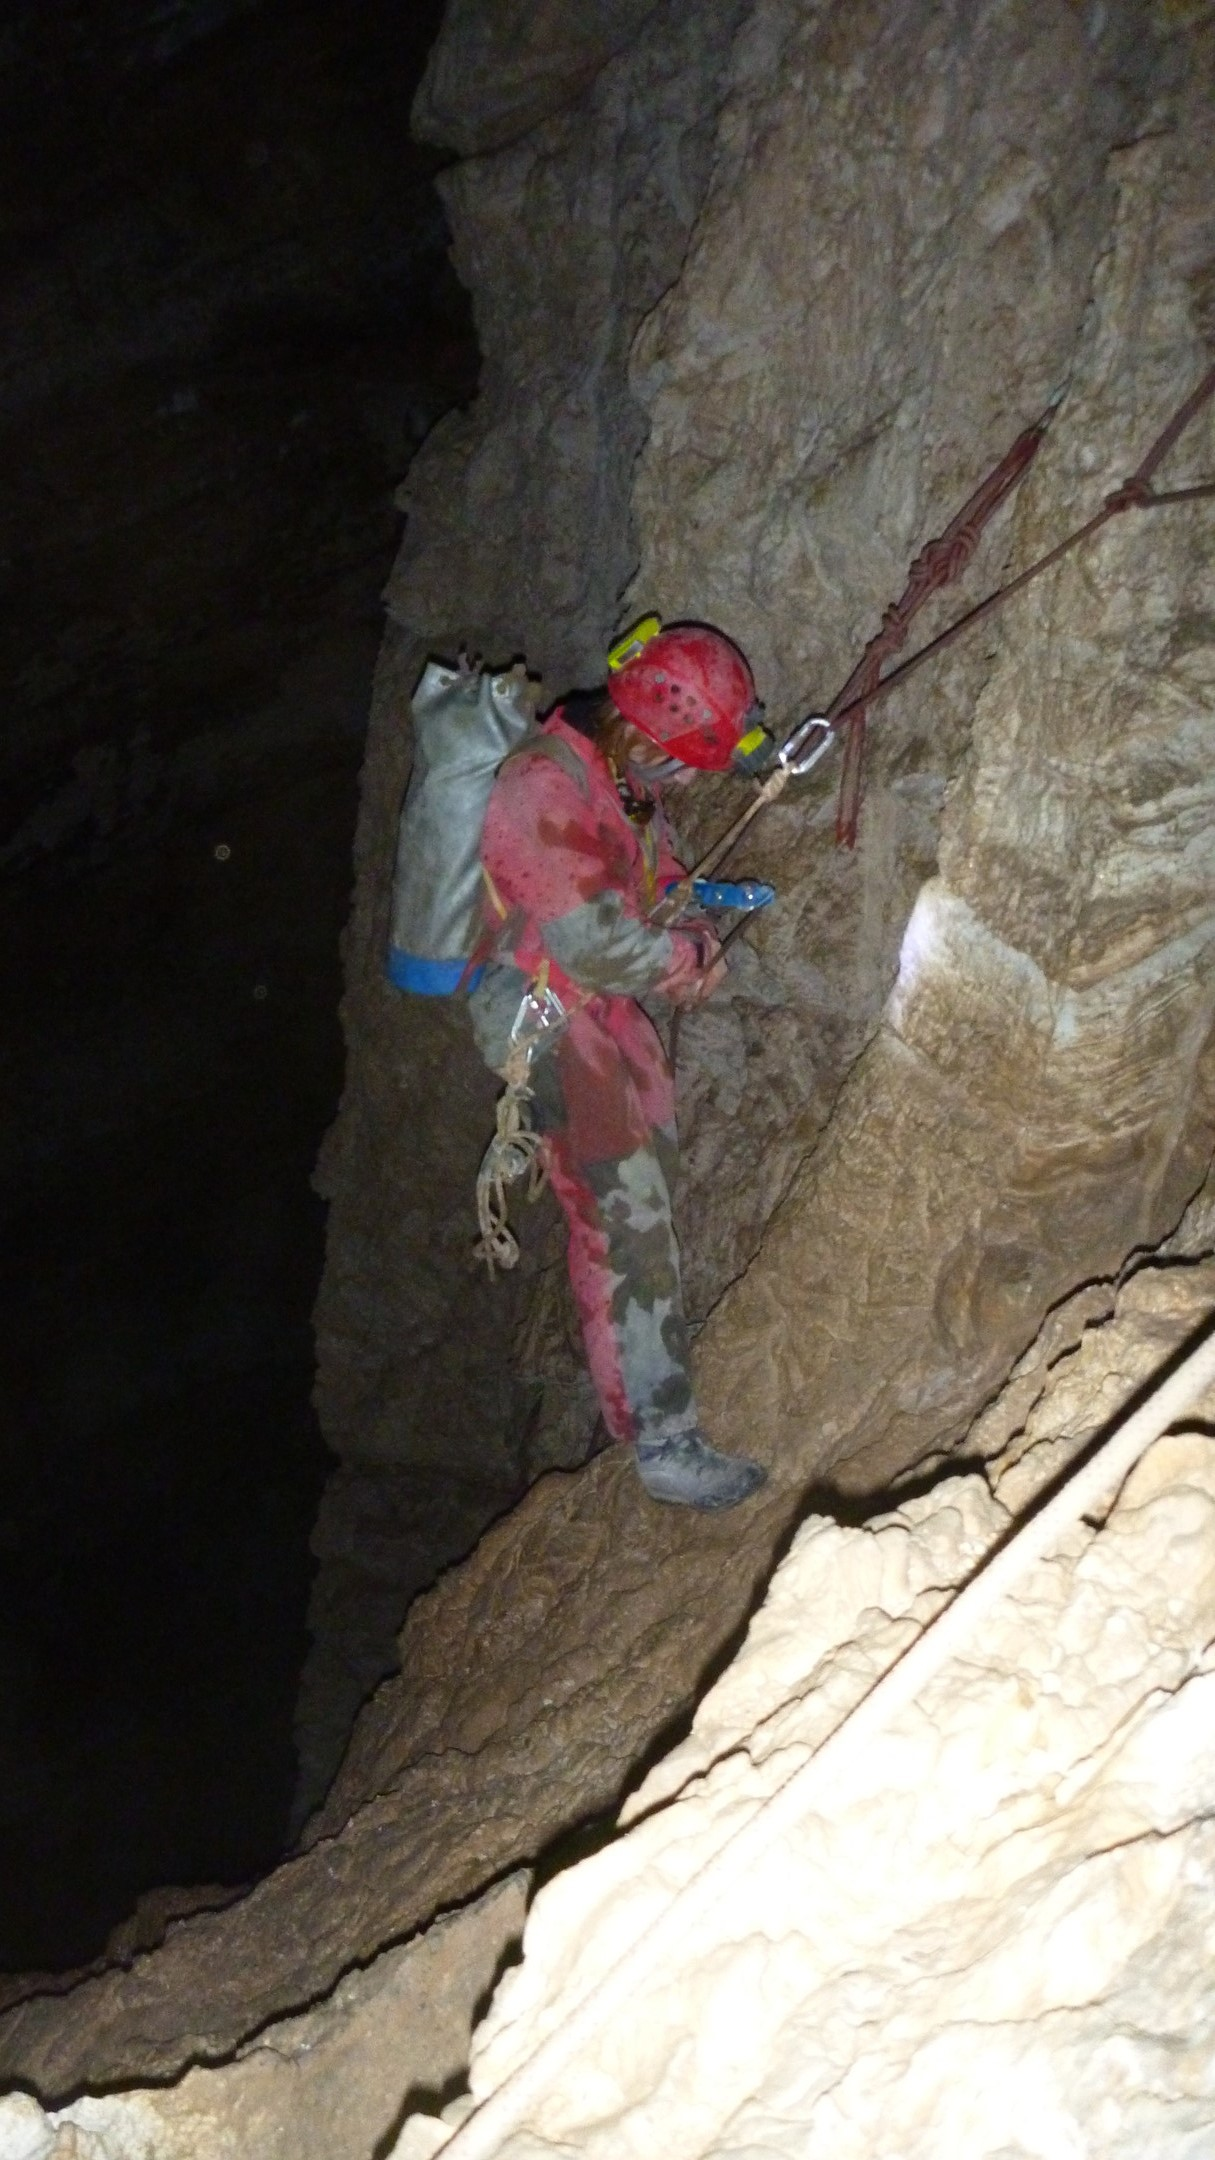
\includegraphics[width=\linewidth]{2011/winter_journey/2011-08-01-12.50.51-Grega-Panasonc DMC-FT2-078-pico pitch head--orig.jpg}} 
 \caption{The head of \passage{Pico} pitch. \pic{Grega Maffi}}
 \label{pico tjasa}
\end{marginfigure}

Then Samo voiced his agreement, and it was up to me. I hesitated; I'd
already made plans for a fun, relaxing jolly to \passage{Pico} with Kate
and Nia\ldots{} and Tetley's proposal was a trip of a very different
nature indeed. But the cave was calling. I thought of the lead we'd left
in \passage{Daydreamers} on our previous trip, the promise of extra depth,
the uncertainty of what we'd find below the next pitch\ldots{} And I was
all too aware, as I am sure Tet was too, that this might well be the
last opportunity of the expedition to push the deep stuff -- the
\passage{Republika} streamway and the \passage{Insomnia}/\passage{Daydreamers} series
below it are not places you want to be when the flood pulse hits. I
looked out of the \passage{Bivi} to the same blue sky and bright sun I woke up to.
Fuck pleasant bimbles, I thought, I'm going down.

``When do you want to leave?''

``As soon as possible,'' the Sly One grinned back. It crossed my mind
that he knew I wouldn't---couldn't---have said no. I take the piss a lot
about Tet's `boys' and manipulations and games within games, but the
bottom line is caving with Tetley is just fun.

And so, by sheer serendipity, utter jamminess of being in a particular
place at a particular time, I found myself on yet another storming
camping trip. It's interesting how much chance affects who you cave with
and which trips you do. Neither of us had planned to cave with the other
again this expedition and yet there we were, at the entrance to
\passage{Vrtnarija}, ready to face the darkness once more.

``Well,'' one of us said, ``here we go again.''

Tetley in front, we both danced down the pitches, comfortable with the
pace, knowing where to place our feet at each rebelay and the little
quirks of each pitch head. \bignote{I savoured the rare feeling of competence};
the back and forth of ``rope free!'' and ``okay!'' that I'd come to
associate with expedition caving. Innocuous though it may seem, I
remember thinking: this is one of the reasons why I love caving.

We soon reached camp, and there we shared a congratulatory brew with
Gergely and Izi, who had just pushed 500 m of storming horizontal
passage (below \passage{Stuck in Paradise}). We chatted excitedly about the
new leads for a while, but we were on a mission and time was marching
on\ldots{}

Once we finished packing our tacklesacks for the second part of our
journey, we bid them goodbye and set off. The deep, horizontal stuff
below \passage{Big Rock Candy Mountain} has some of my favourite caving in
the system. Not unlike Welsh caving at its best, the meandering rift
passages of \passage{Highway 32} or labyrinthine tunnels of the \passage{Leprechaun} series
possess a distinct, individual beauty; its existence alone this deep in
an alpine cave system is incredible.


\margininbox{Daydreamers}{
     \begin{itemize}
    \item James "Tetley" Hooper
    \item Clare Tan
    \end{itemize}}{\explo}

We nipped along the passage, familiarity making the journey pleasant.
Before long we were back at \passage{Republika}, then \passage{Insomnia}, and finally
the cascades of \passage{Daydreamers}. I love returning to little bits of
cave I've pushed. It was wetter than before, but the water levels were
still safe enough. We established `base camp' in a little sandy alcove,
picking up a bottle of meths and a mess tin along the way---remnants of
a sneaky little outpost that Tetley and Samo set up in \passage{Republika} two
years prior.

Tetley started bolting the pitch, and serenaded by the `tap, tap, tap'
of hammer against driver, I busied myself heating up a tin of tuna with
the meths, and brought out the slices of fresh bread, transported
carefully down in a Daren drum.

``Would you like the sandwich there, or are you coming back here to
eat?'' I shouted down the passage.

``Here, please!''

So there we were, 840 m underground. Myself, clipped into the traverse
line, legs dangling over the lip of the pitch, and Tetley, a metre below
me, swinging about on the rope midway through his second bolt, each
enjoying a hot tuna sandwich. And what a sandwich it was! What luxury!
Princes Tuna in Sunflower Oil, king of all underground edible
matter\ldots{}

Then---``Do you think you could roll me a fag?''

``Sure. Well, I'll try my best\ldots{}'' Unbidden, \bignote{the memory of Myles
prophesying that rolling is a life skill that will one day come in handy
came to me}\ldots{} Don't drop the bag, don't drop the bag, I told
myself. I knew Tet would kill me if I lost his baccy. I rolled a
passable cigarette, lit it, and he disappeared down the pitch. I, of
course, followed.

\passage{Daydreamers} continued in the same vein for a while, short 5--15
metre cascade pitches which we took turns bolting. How it teased us!
Would it go? Would it sump? Never knowing what exactly we'll find around
the corner, a thrill of exploratory caving I doubt I'll ever grow tired
of. Eventually, the last pitch we dropped turned out to be a blind one.
The water gurgled mockingly into a ten centimetre wide, angled bedding
plane rift, and we were unable to follow it.

I couldn't help but feel a little disappointed, suddenly becoming more
aware of how cold it was\ldots{} Camp \passage{X-Ray} and hot, sugary tea
seemed far away. Tetley, perhaps sensing my deflation, offered some
consolation, ``Don't worry, we'll find a bypass!''

I grinned back. This was still a stonking good trip, regardless.

``On station!'' We began to survey.


\margininbox{Penguin's Egg}{
     \begin{itemize}
    \item James "Tetley" Hooper
    \item Clare Tan
    \end{itemize}}{\explo}

Though our callout was beckoning and we still had surveying to complete,
we knew we couldn't leave a quasi-lead hanging like this, not when the
pushing front was so far from camp. So we pushed on through an old
fossil level that continued above the blind pitch, which I'd explored
briefly while Tetley was bolting earlier. It didn't look too promising,
but it kept going, so we went with it. With each metre gained in the
abandoned bedding plane, I allowed myself to hope a little more. But \bignote{the
higher one's hopes, correspondingly, the greater one's fear} of killing
the lead. Such is the paradox of deep cave exploration. It is both a
blessing and a curse, and I would not change it for the world.

Finally, we got to a roomy chamber with the unmistakable rumble of water
in the distance. I flashed Tetley what I'm sure was a jubilant grin. It
seemed as good a lead as any to leave; we shook hands, and the whole dry
series we named the \passage{Penguin's Egg}, for:

\begin{quote}"If you march your Winter Journeys you will have your reward, so long as all you want is a penguin’s egg." \end{quote}

\name{Clare Tan}

\newpage
\section{Winter Journey}

\begin{marginfigure}
\checkoddpage \ifoddpage \forcerectofloat \else \forceversofloat \fi
\centering
 \frame{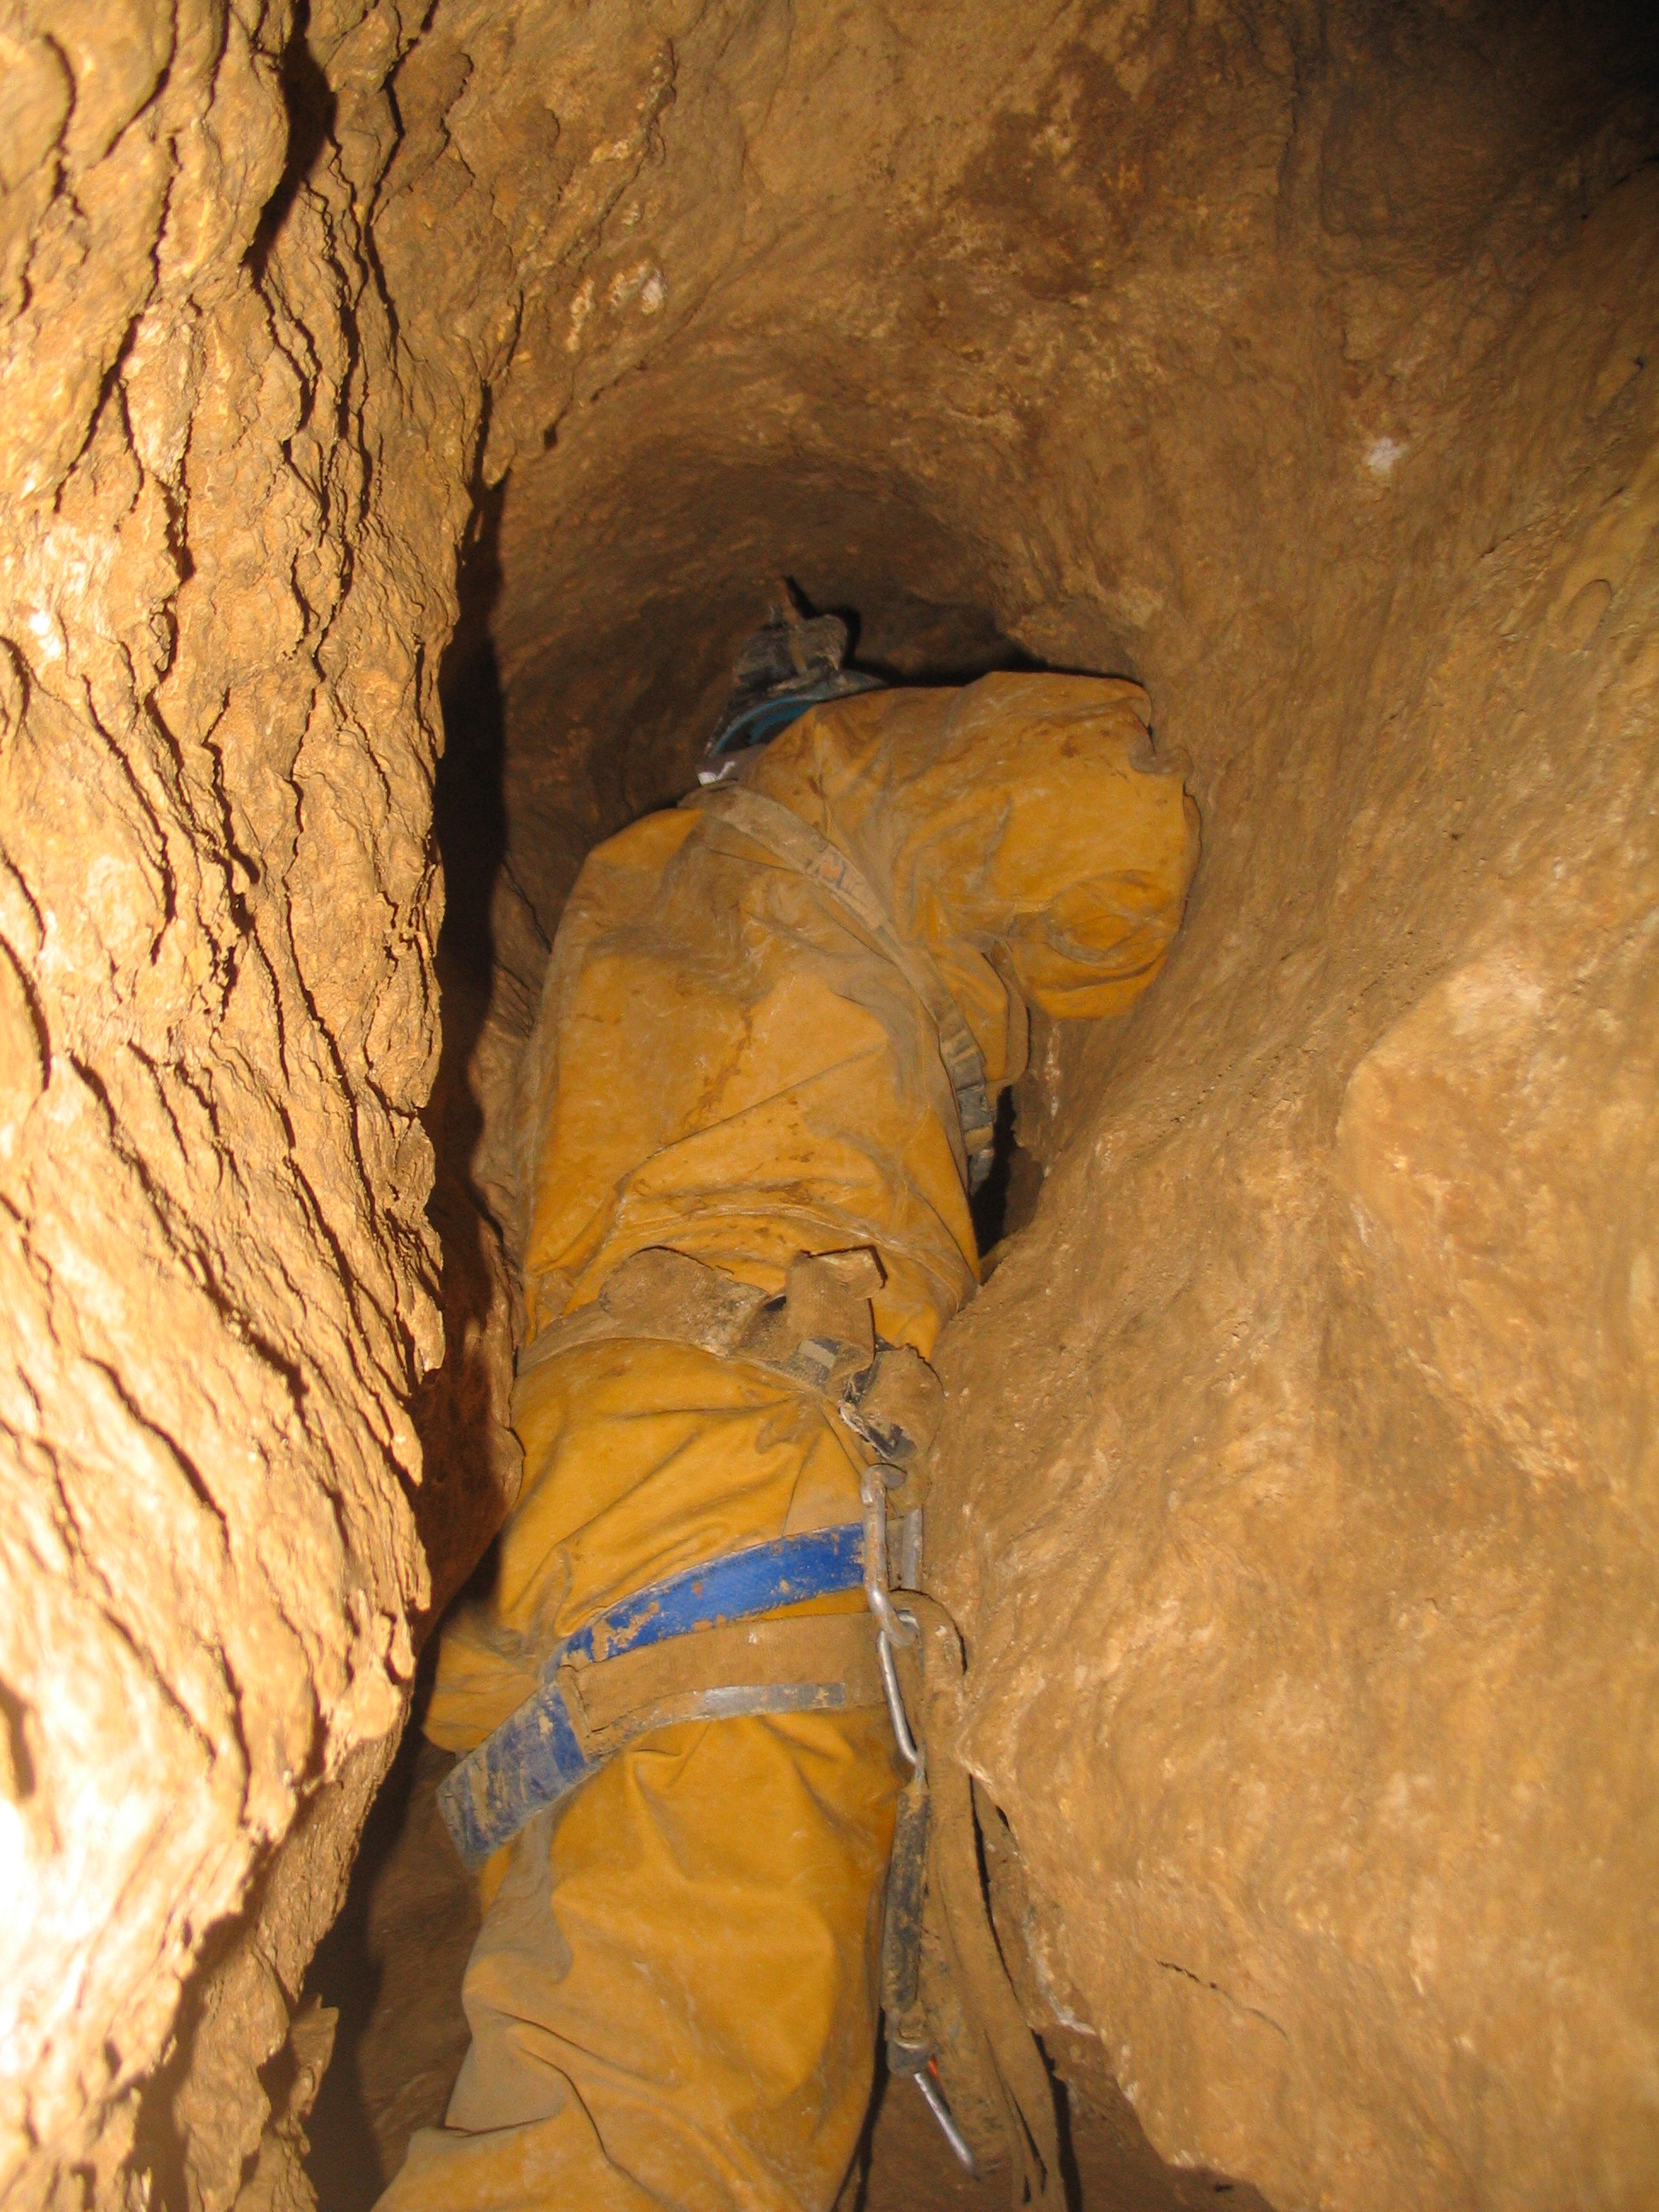
\includegraphics[width=\linewidth]{2011/winter_journey/20100801-16-19-15-Jarvist Frost-Canon G5-IMG_0413-Cascade beyond Black Knight duck and Sidewinder--orig.jpg}} 
 \caption{\passage{Sidewinder} led to \passage{Crack in Time} and a connection to the passage \passage{Envy}, which is deeper than \passage{Big Rock Candy Mountain}. \pic{Jarvist Frost}}
 \label{jana sidewinder 2010}
\end{marginfigure}

I have never been to the `deep' part of \passage{Vrtnarija}, below
\passage{Big Rock Candy Mountain}. Or rather, I was with Jana when we
pushed \passage{Korita} to a connection, and free climbed down from an unlikely
rift in the ceiling (`The \passage{Crack in Time}') to reach \passage{Envy}. That tiny taste
of dry, ancient, phreatic as I continued down the crawl ways solo to
find a PSS left a ticklish taste in my mouth. Such a strange, quiet
place.

Time on expedition was running out, so if I was going to get down
\passage{Big Rock Candy Mountain}, it had better be soon! Jim Evans was
recently up on the mountain, but rather lacking in terms of warm
clothes. It later turned out that he'd forgotten he'd sent out a bundle
of his warmest technical garments in the minibus, and had thus failed to
find them when he flew out. They were safely sealed in a barrel at
\passage[town]{Ravne}, while he shivered up top.

But he was up for a deep camping trip.

Clare and Tetley had headed off in the good weather at the morning, Jim
and I were taking rather longer to get ready. As the slower party of the
day, we had, by default, drawn the short straw and committed ourselves
to a `night train'. By the time we were thinking to go, Andrej had
arrived. He was interested in \passage{M2}, but as there were few
experienced cavers left on the mountain top, he very readily converted
to \passage{Vrtnarija}.

And so we were off, what a fine collection of Speleologists to be going
deep with, I am caving with the very pioneers of deep exploration on
\passage{Migovec}! Jim is having to remember a fair bit of SRT as he goes, but we
make steady progress to camp, saying hello to Mike and Ari at around nine
in the evening. Apparently Tetley and co. are not to be expected for a
considerable time, which makes us rather worried about how strict they
were intending to be with their Day Train booking in the camp roster.
Now as a 3-person team, we have less flexibility if Tetley and Clare end
up between the tracks.

\margininbox{\passage{2nd Time Lucky}}{\textit{4/8 -- 10:30 ish} --
Mike + Ari. Have just eaten my body weight in couscous (Dave declined b/fast) and am both Happy+Sad. Off to go caving down the push on \passage{Friendship Gallery} soon. \name{Mike}

\textit{5/8/11 9am} -- Mike + Ari: below \passage{Lower Pleasures}, ``\passage{2nd Time Lucky}''

Went back Fr. am to drop our pitch with correct length rope. Epic faff
on my part which Ari did well to put up with. Two windows down pitch. 5 m drop with water at bottom and rift going over 5 m drop. Tightish but air fresh -- no draft. Sorry Ari! \name{Mike}}{\logbook}

\passage{Big Rock} is a truly stupendous pitch. It's absolutely lovely. I eagerly
checked out the window on the far side of the rift. It leads through
onto an absolutely massive chamber, almost that we're descending in the
side shaft. Tetley's Spaghetti, where rope thrown from the top of the
pitch ended up impossibly tangled halfway down, I had assumed was Dave
and Jonny's newly rigged drill traverse. I was later told that in fact,
this rope isn't properly belayed at all, and that Dave took out their
piece of rope again. Quite glad that I didn't attempt to get on it!

The conglomerate rock on the floor of \passage{Big Rock Candy Mountain} is
very interesting, specs of black, suspected Haematite, glued together
with an open sponge of limestone chips. Andrej and Jim soon join me. It
is here that our trip starts to go slightly astray.

``Oh, I think my concussion is coming back!'' groans Fratnik, his helmet
off, exposing the large wound where he was knocked off his mountain bike
earlier in the week.

I look for Jim, he's down near the little stream with his water bottle,
I assume making the best caving use of a stream, in having a piss and
drinking some refreshing water. I do a double take -- he has his penis
inserted into the wide mouth of the water beaker (as I find out later,
the bottle was carefully selected for this very purpose), he then tops
up with fresh water and drinks from it.


	\begin{figure*}[t]
	\checkoddpage \ifoddpage \forcerectofloat \else \forceversofloat \fi
		\centering
		\begin{subfigure}[t]{0.49\textwidth}
			\centering
			\frame{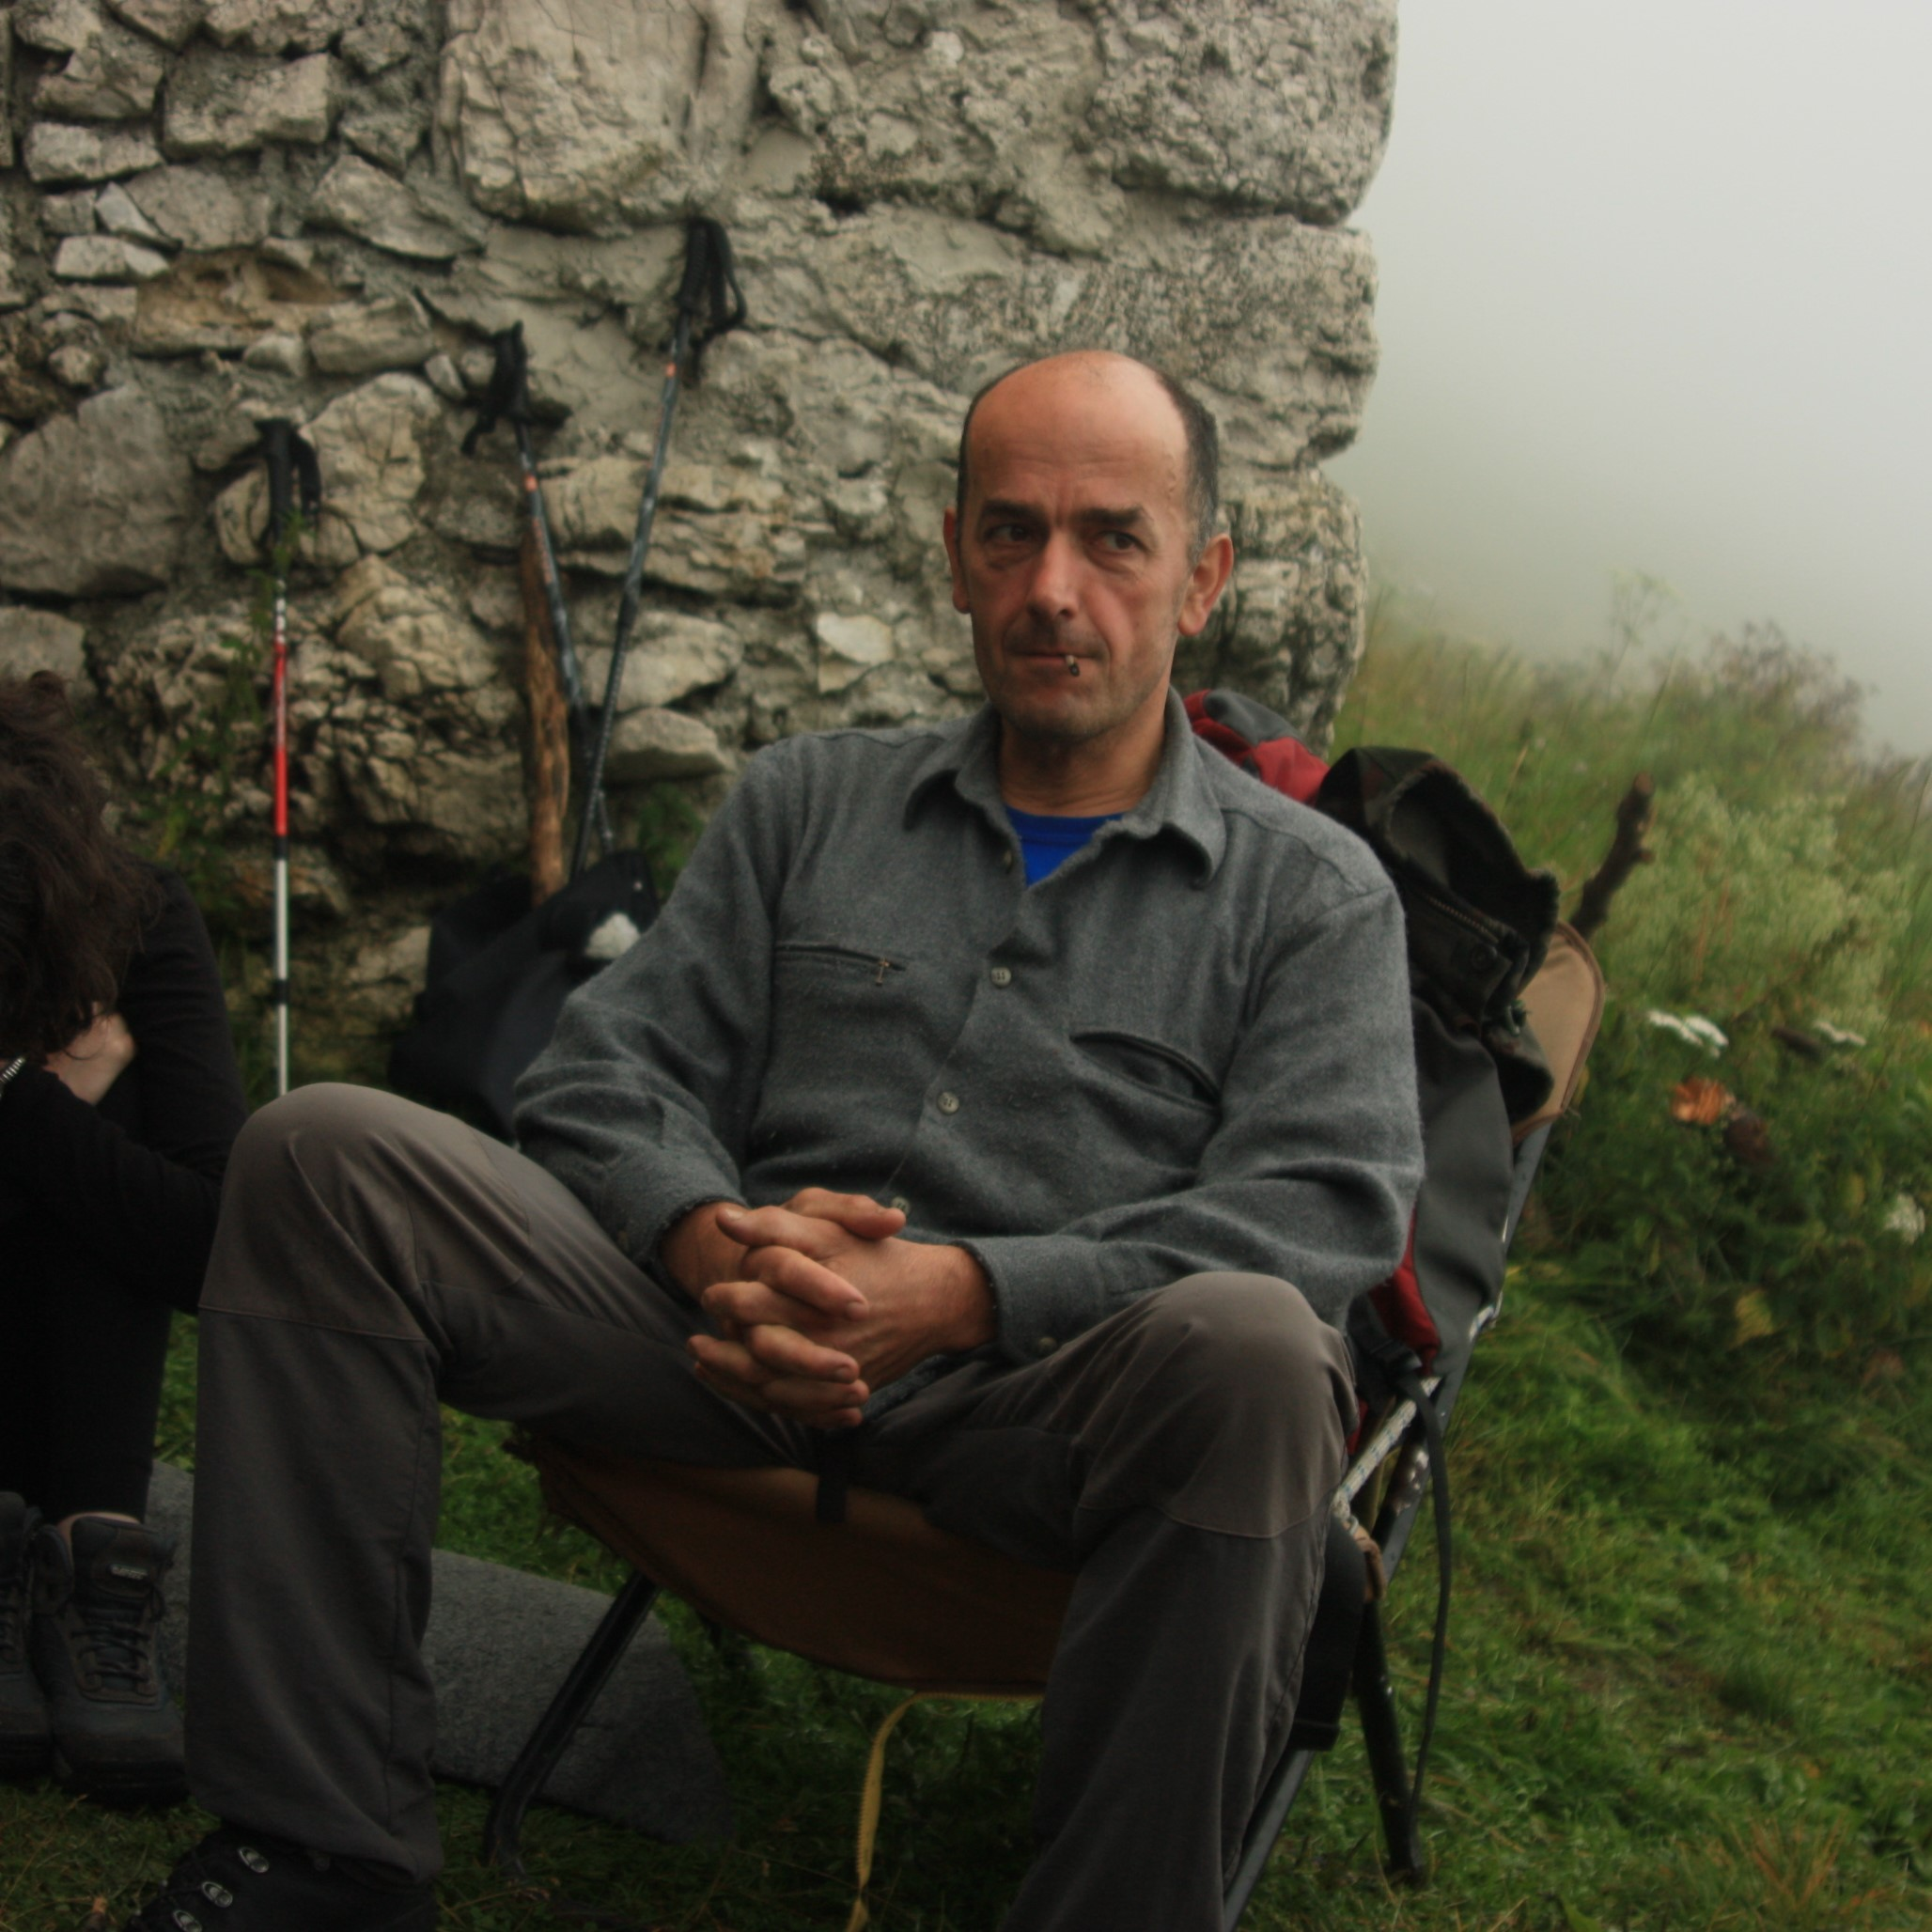
\includegraphics[width=\linewidth]{2011/winter_journey/2011-08-07-09.17.29-Gergely Ambrus-Canon450D-IMG_1207-Zdenkos 50th Birthday Party at Kal--orig.jpg}}
			\caption{}
			\label{fratnik kal}
		\end{subfigure}
	\hfill
		\begin{subfigure}[t]{0.49\textwidth}
			\centering
			\frame{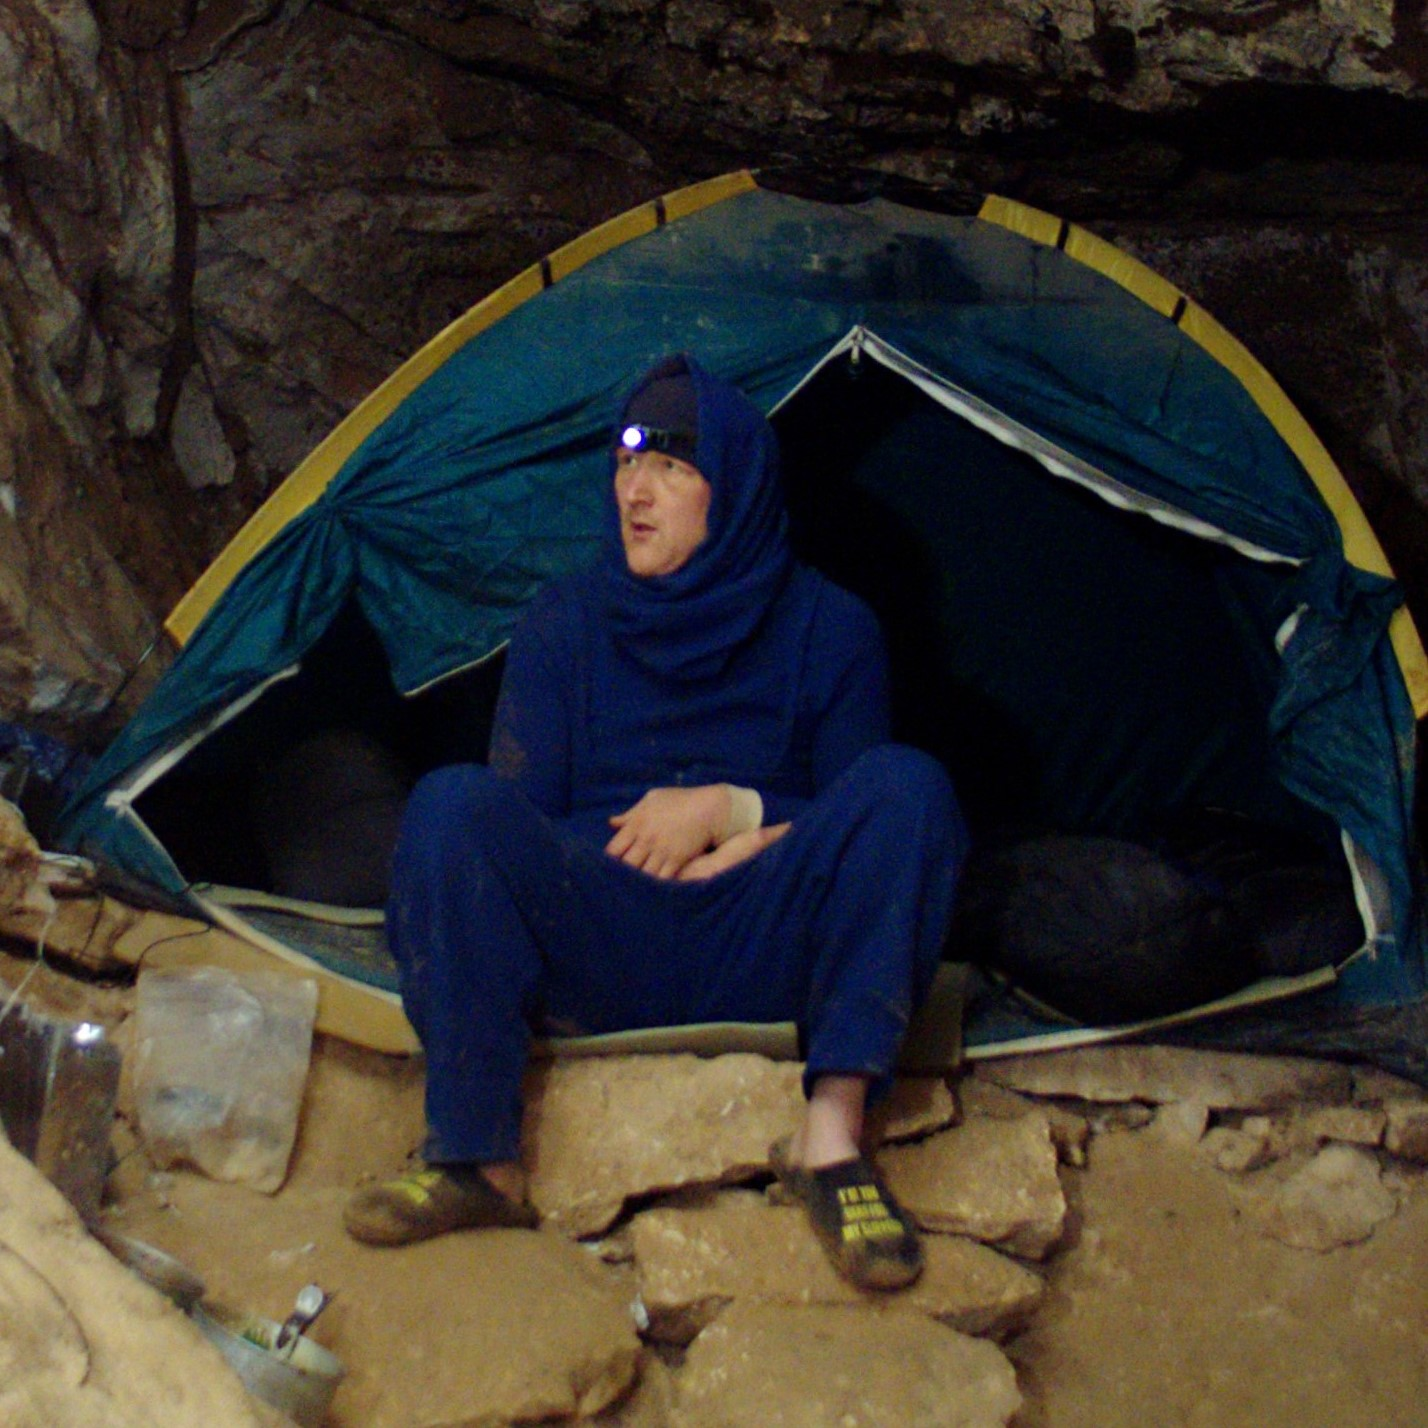
\includegraphics[width=\linewidth]{2011/winter_journey/2011-08-07-12.02.38-Jarvist Frost-CanonG5-CRW_0170 - jim at camp--orig.jpg}}
			\caption{}\label{jim x-ray}
		\end{subfigure}
		\caption{Two of the pioneers of \passage{Migovec} exploration.
  \textit{(a)} Andrej Fratnik at \passage{Planina Kal}. \pic{Gergely Ambrus}
  \textit{(b)} Jim Evans, -550 m below at Camp \passage{X-Ray}. \pic{Jarvist Frost}}
	\end{figure*}


Wow. Minus 650 and all is well.

Navigation soon became rather difficult. Jim and Fratnik have both been
here before, but memories fade. \bignote{Luckily we had stolen the A3 laminated
survey from UG camp as we passed through}, and this became rather useful
in combination with our survey compass.

\margininbox{For Evans' Sake}{A special lifetime achievement award for Jim 'Drink your own' Evans, for long standing services to experimental medical science in the utilisation of bodily fluids.}{\award}

From \passage{Big Rock Candy Mountain} you can follow the stream,
traversing above the trickle of water (\passage{Highway 32}). The rift is high,
and on the way back I ended up doing some crazy free climb back down at
the end. Continuing into the cave you reach a sandy oxbow, with a lake
to the left, which I assume is the source of the little stream that
disappear down at the far side of the oxbow (and, one assumes, forms
\passage{Brown Rice Inlet}). It's an interesting area, and one that would be worth
checking out seeing how this `\passage{Highway 32}' interacts with \passage{Big Rock
Candy Mountain}. We blunder directly into what I believe is `\passage{Postiga}',
and end up looking down into a chamber with what look like footprints,
but for which there is no way down.

Backtracking, Andrej remembers that you have to double back to camp\sidenote{\passage{The Fridge}, the 2004 expo's underground camp}. We soon find the rope leading down.

Down into a maze of twisty tunnels. Unfortunately, very few PSSs were
placed in this area, and it's only when we pick up the `\passage{Mad Cow}' PSSes
left by Andy and Rik on their accidental resurvey\sidenote{also a 2004 adventure} that we know we're on
the right track.

Once out of the small crawly bits of \passage{Leprechaun}, and having found the
subtle `hidden under a ledge on the right' pitch down, the passage
develops into a very curious large phreatic. Andrej comments that he
reckons the water never ever flowed here, just percolated away leaving
all this silt in place. Certainly there are no obvious stream features,
but the few pitches and climbs could be old cascades.

\bignote{The rigging gets more inspired}, and rather minimalist. After a very
strange traverse-pitch in a amphitheatre-like corner of passage, we dive
through the sandy digs and `thomp, thomp, thomp' our way to what is
clearly \passage{Red Cow Roundabout}. There's a bundle of old rope here, and an
inviting crawlway leading off to the right. With wide passage, plentiful
sand, accessible water and little draught, \bignote{this would make a very nice
camp} at -736 m.

We regroup, then head down the inviting crawlway. Soon we reach the
little pitch and stream, I know this must lead quickly to the original
\passage{Red Cow} sump but stupidly I don't go and have a quick look at it,
instead heading directly upstream to \passage{Republika}. We were more
than a little bit worried at this point, as Tetley and Clare were meant
to be on the Day Train -- but it was already past midnight. Were they
alright?

In the little crawlway above the stream I hear voices ahead, and sit to
wait until Tetley and Clare show up and Andrej and Jim catch up from
behind. It is now well gone midnight, they won't be returning to camp
till 3 or 4AM at least. Their Meanders glisten with water, \bignote{they are
upbeat but their wild staring eyes speak a slightly different story}. To
be honest they are a little short with us, considering they are the ones
transgressing their Camp \passage{X-Ray} booking, apparently just due to
exploration fever. They relate their latest discoveries: the original
streamway lead is dead, but an abandoned bypass into a chamber has been
found. We agree to leave them sleeping till Noon at least, and bid them
well.

Onwards to \passage{Republika}, up a free climb next to the stream. The
chamber is not too heavily spray lashed, by traversing you can avoid the
twin waterfalls coming in from up high. I have a good look at the
ceiling. The original description water being split on a boulder is not
quite correct, it's more that you have water entering at opposite ends
of a massive rift, and the \passage{Republika} chamber is where these two
separate routes of erosion have happened to intersect (I'd suspect). The
bigger waterfall certainly seems to be the one that feeds the \passage{Red Cow}
sump, but it's difficult to assess the flow rate for certain.

\passage{Republika} pitch is rigged with what must have clearly been a
speedy minimalism, almost all naturals, with a crazy rebelay in
freespace dangling off a sling looped over a rock bridge. As a result,
the hang and rebelay are wet, but it could be rigged perfectly dry
(after bolting!) with an easy traverse on the large ledge.

Next we know is \passage{Insomnia}. This has a profusion of stainless 8 mm
rawl bolts, and no naturals, yet still is rather terrifying in its own
way! James KP is very tall, abseiling down onto the swinging traverse
rope that crosses the pitch about 2 m off the ledge is rather a
challenge to execute safely, and the single bolt providing the hang for
straight down the 32 m pitch is terrifying. Halfway down the pitch there
is a bouldery ledge that could be easily gained, and may have some
\passage{Kamikaze}-like lead running off it. The bottom third of the pitch
is potentially very wet. Going down you can easily traverse sideways
with your feet, on the way back up you have to self-deviate with a spare
hand to the pitch wall to avoid swinging out into the spray.

Below \passage{Insomnia}, you are in a classic bit of stream cave, could be
anywhere in Yorkshire as you clamber in crawl-ways above the water. The
last item in \passage{Insomnia} is a hand line on a toboggan, which would
be rather entertaining in the proper wet.


\begin{marginfigure}
\checkoddpage \ifoddpage \forcerectofloat \else \forceversofloat \fi
\centering
 \frame{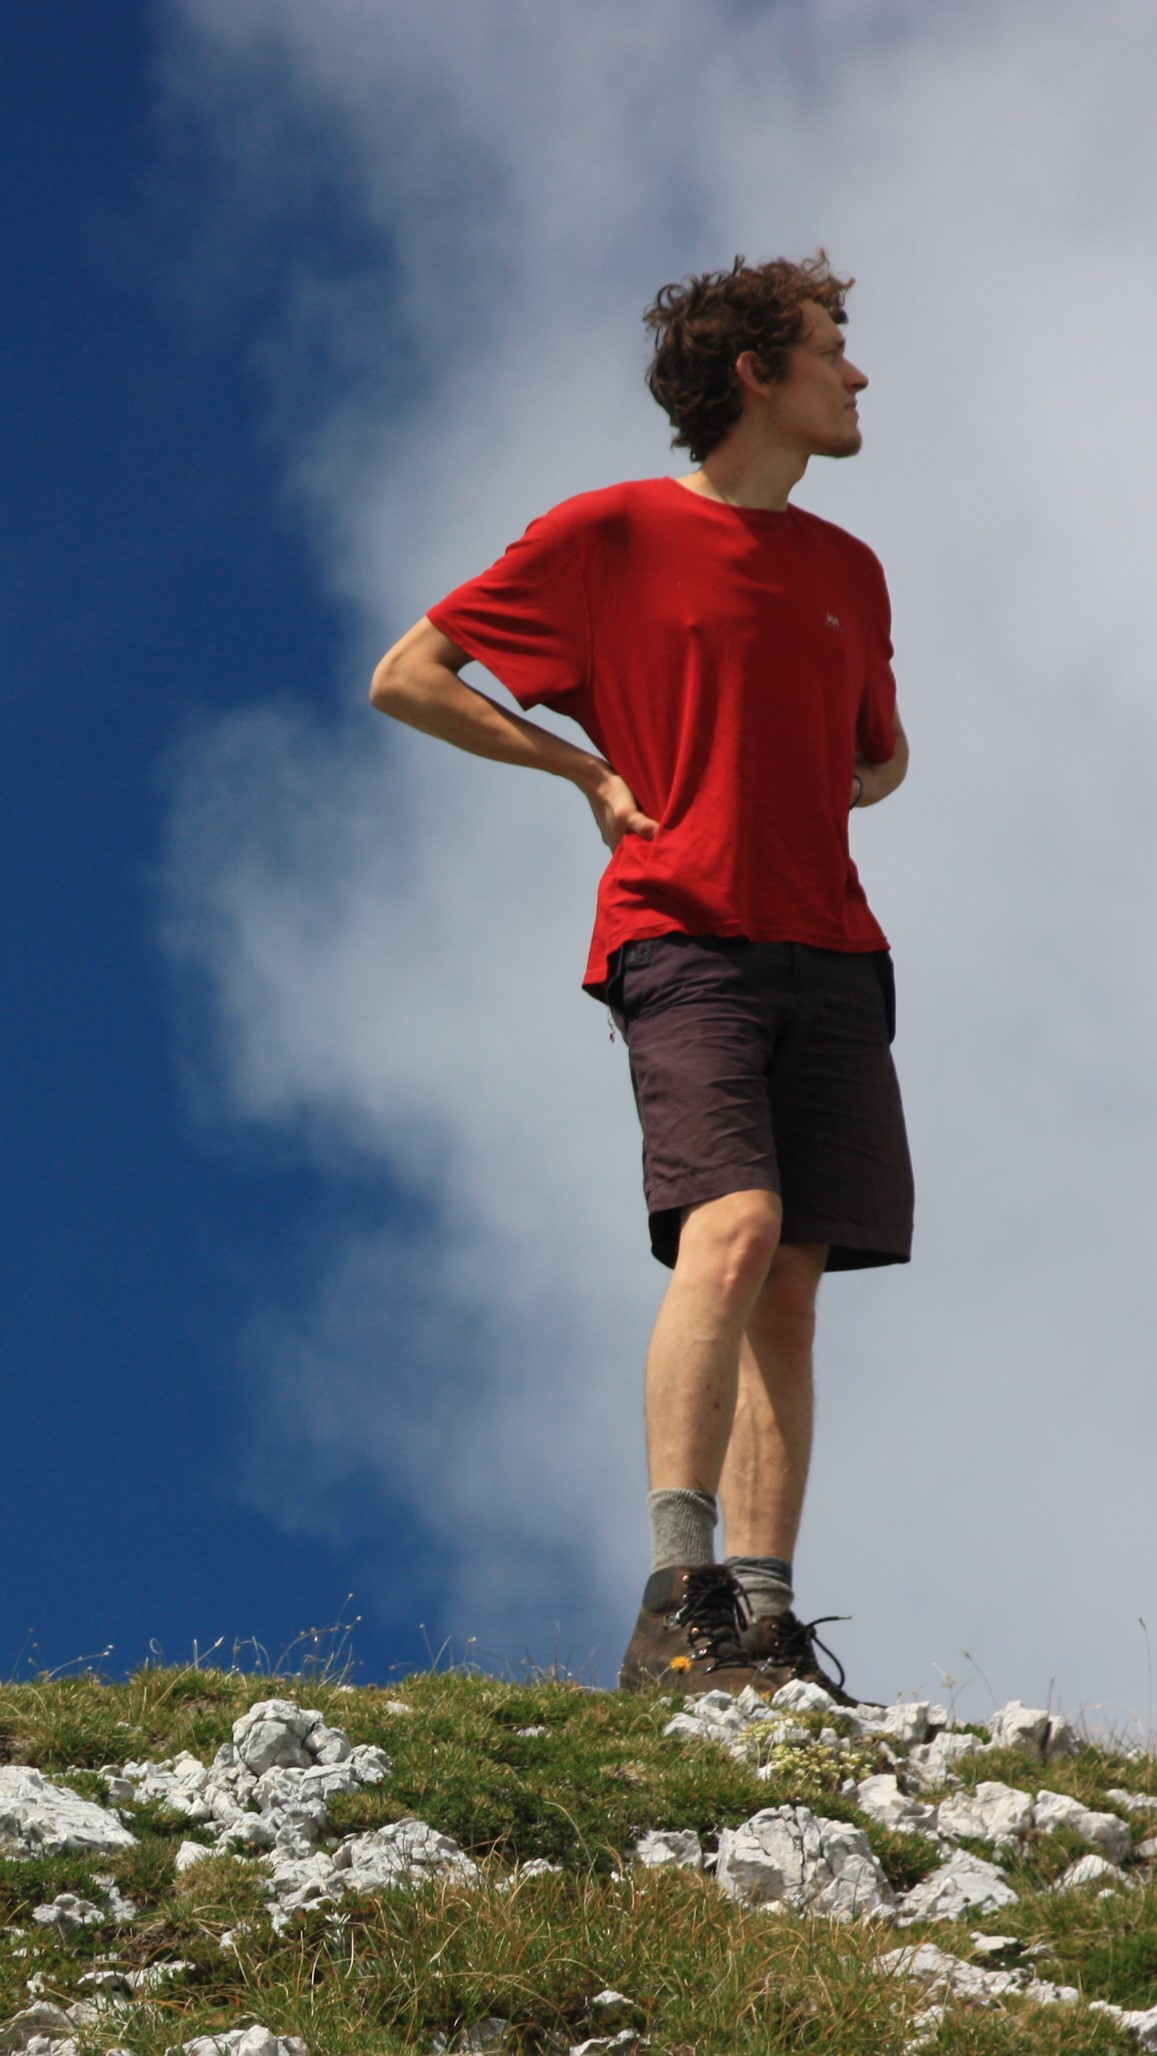
\includegraphics[width=\linewidth]{2011/winter_journey/2011-08-02-11.42.37-Gergely Ambrus-Canon450D-IMG_0829-Walk up Kuk--orig.jpg}} 
 \caption{Jarvist in warmer climes, on the slopes of \passage[mountain]{Kuk}. \pic{Gergely Ambrus}}
 \label{jarv kuk}
\end{marginfigure}


Soon into the \passage{Dream} series, we drop a number of little 10-15 m pitches,
always near the water. It's great fun, and would be an excellent Grade
III in Yorkshire. With such cold water and so far from a place of
safety, it's rather more sobering here. The hang from one of the rifts
doesn't go quite far enough at one point, leaving you suspended above a
deep pool. I kick off the wall behind and try to abseil down in one
quick manoeuvre, but don't quite get enough slack through and swing back
dragging my heels through the water. My wool socks are soaked, and my
feet will be freezing till I get back to the surface.

Finally we reach a long hall dipping down at about 20 degrees, rope is
necessary but you sort of abseil by climbing off opposite sides of the
rift. There is a crazy dumbbell shaped rock sitting nonchalantly on a
shelf, looking utterly artificial.

Finally the water disappears down a crack in the floor, and the
human-sized route forces you up onto a ledge. A short, unrigged, pitch
leads down, to rejoin the water before it disappears into an impossible
rift, the end of the Dream.

We stop for lunch, we don't have much. A few tins of fish and the bread
from the \passage{Bivi} that Clare and Tetley didn't take. I pop ahead along the
\passage{Penguin's Egg}, a series of crawl ways through muddy layers and down
dipped bedding planes to finally gain the top of a sloping chamber, the
exploration end. I am not filled with massive hope, you can indeed hear
water but the rock and everywhere available surface is covered with fine
grey silt silt, \bignote{the cave feels like it is in shutdown}. Though Tetley and
Clare have certainly left a lead, I can't help but feel that they
themselves would not be in such a rush to come back and push here.

I carefully climb down, past strange grey silt-stalagmites growing out
of boulders, and find my way to the source of the noise.

On the left, a tight rift issues the clear sound of tumbling water, and
also supplies a draught that blows into your face. The too-tight rift is
formed along the dip of the overall chamber, but with a strange
protrusion of rock on the left that stops one from seeing the source of
the noise. I take off my helmet and stick my head in it, no chance of
passing it without significant expansion.

I head in the opposite direction at the bottom of this small chamber
(North), and follow the draught through a series of little muddy
chambers, always at this $\approx$ 60 degree slope of the bedding,
clambering up and down, and sometimes wriggling along sideways. There's
little dry-pools of mud on the flat surfaces, with collections of
colourful pebbles (including lots of little black Haematite flecks) and
banded mud structures.

\margininbox{Winter Journey}{
     \begin{itemize}
    \item Jim Evans
    \item Andrej Fratnik
    \item Jarvist Frost
    \end{itemize}}{\explo}
    
Jim and Andrej arrive, so we press on together. The last little chamber
has a rather more tight slope climb out of it, flat underneath the
inclined ceiling. My head pops out into a more spacious arena and I
realise that the `ceiling' I've just squeezed under is actually a whole
plate of bedrock which has fallen and is now suspended by a mysterious
force. I wriggle out underneath it and into a small chamber. The
continuation upwards leads to an alcove, in the ceiling of which is a
too-tight rift through which I can see draught getting hoovered as I
breathe out condensation.


\begin{pagefigure}
\checkoddpage \ifoddpage \forcerectofloat \else \forceversofloat \fi
   \centering
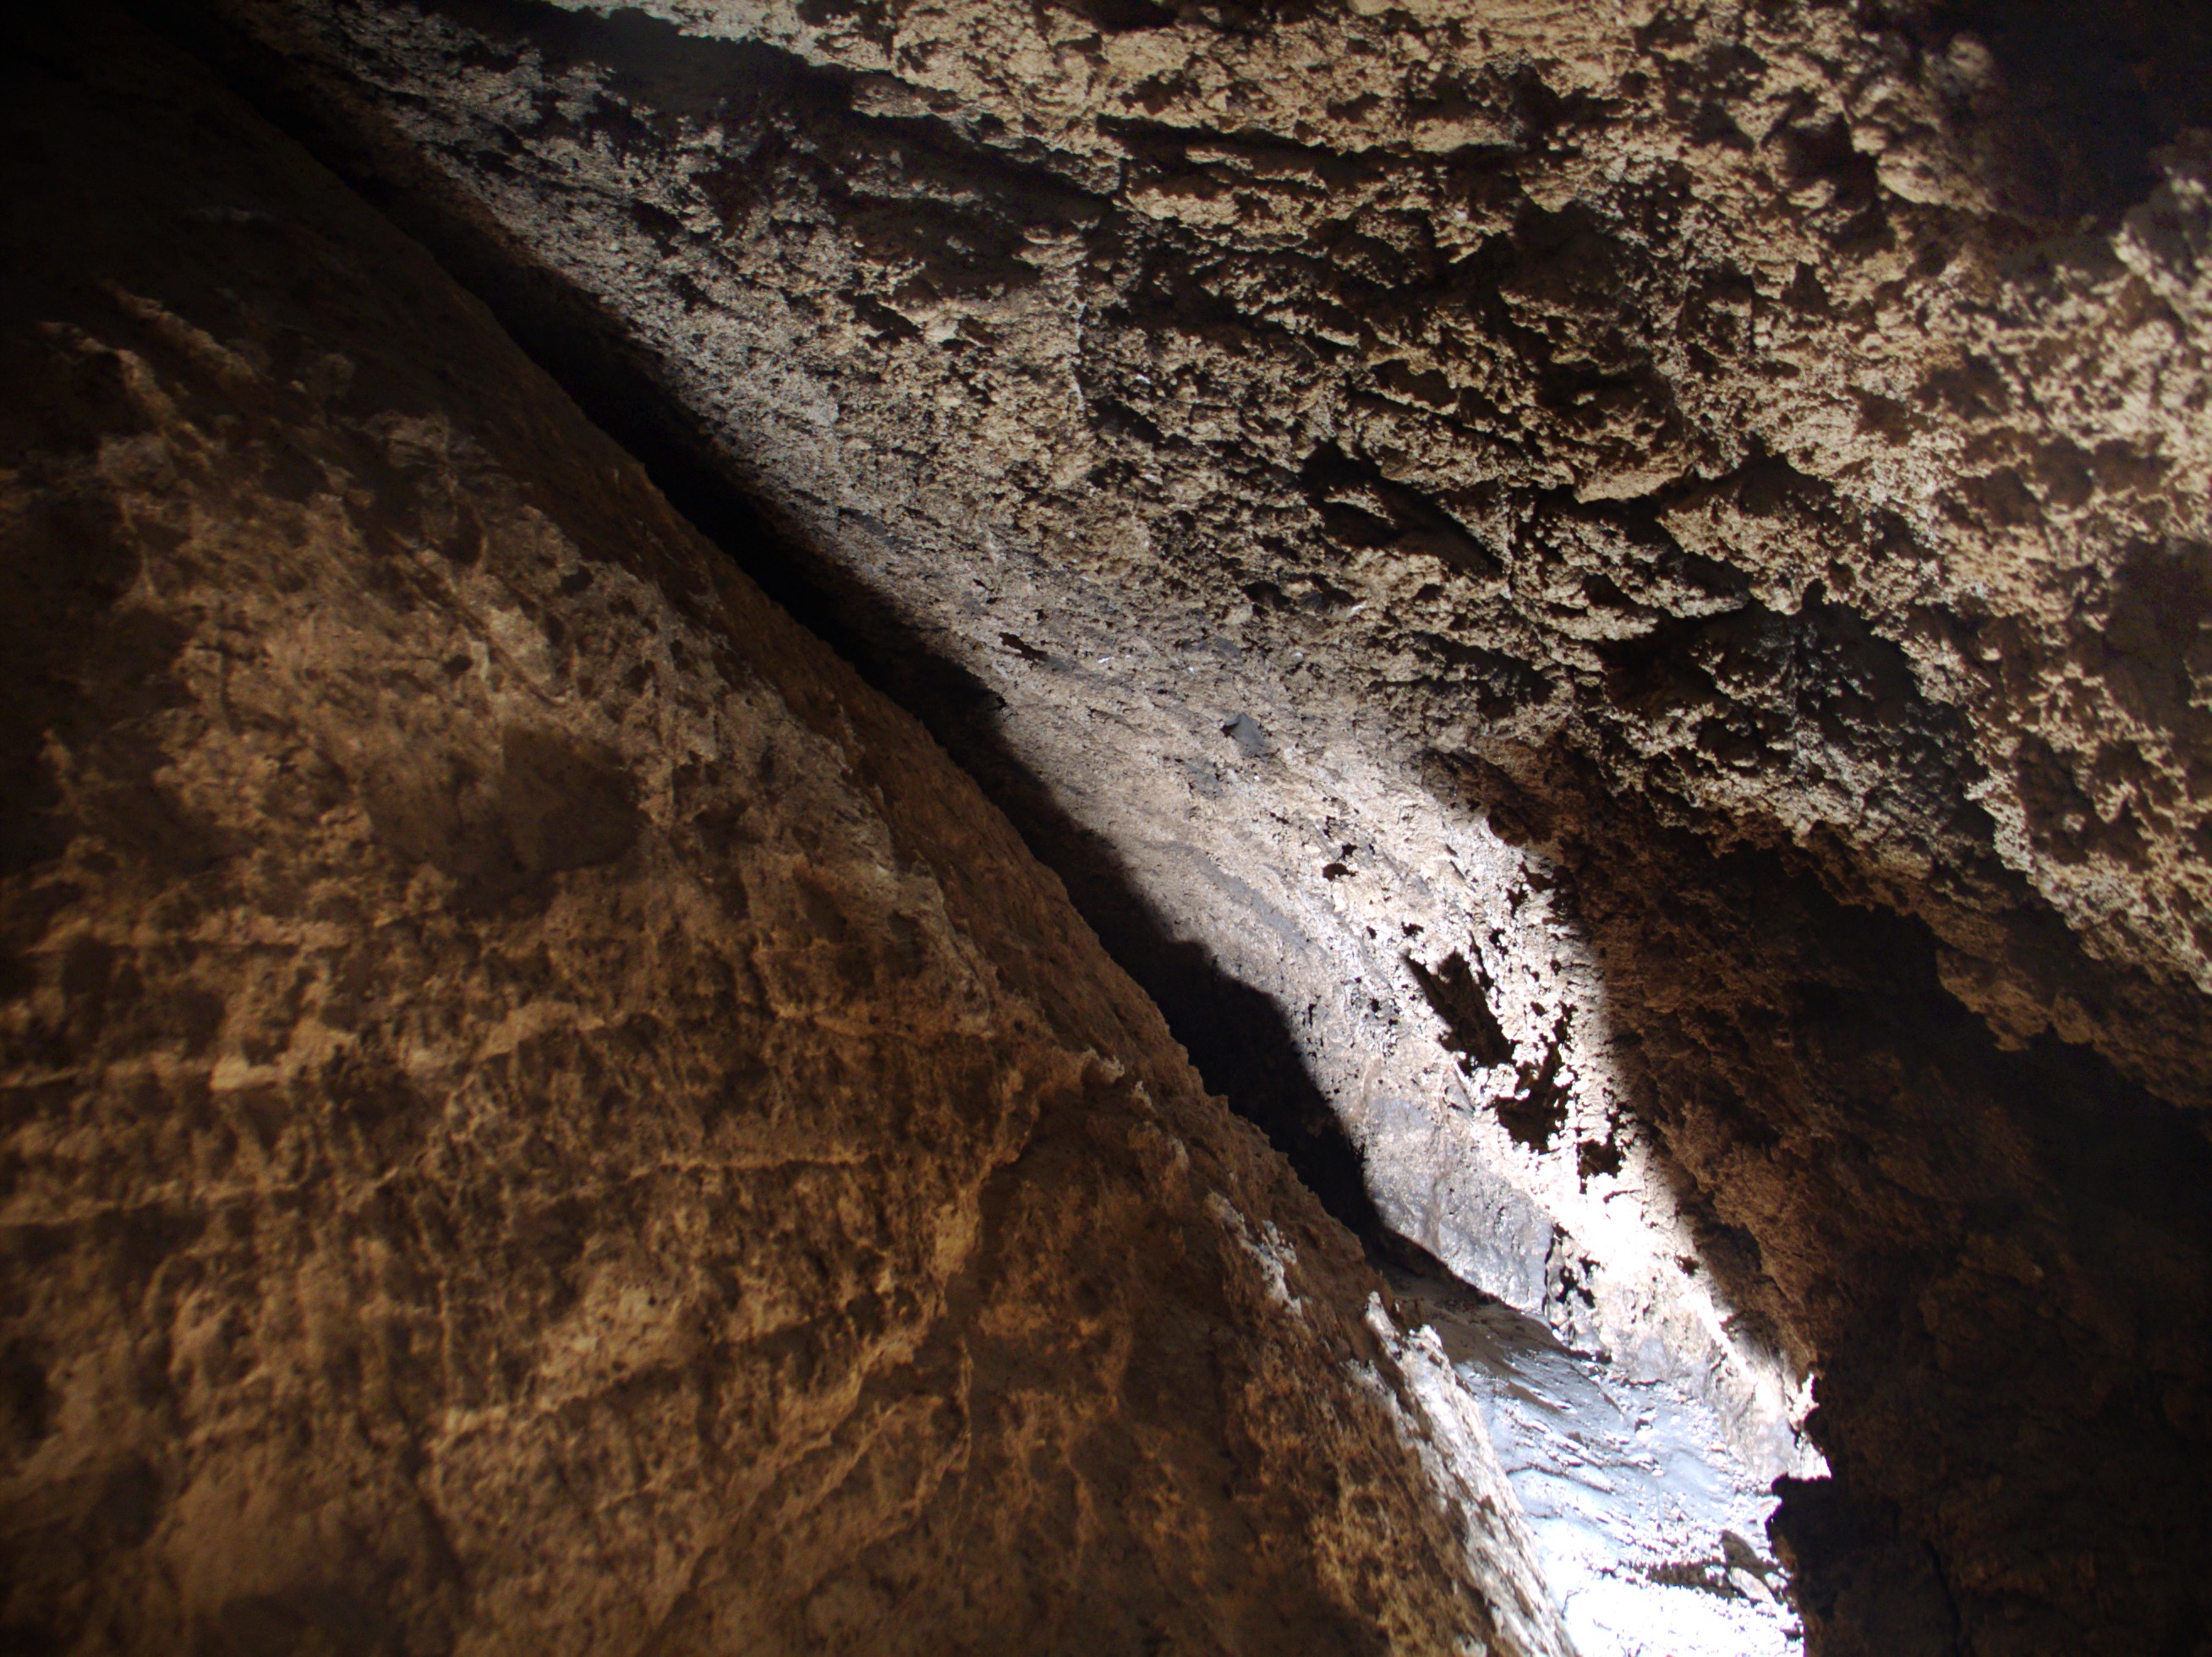
\includegraphics[width = \textwidth]{2011/winter_journey/2011-08-05-03.17.26-Jarvist Frost-CanonG5-CRW_0130 - Terminal Rift - Winters Journey Station Eight - Flash Hidden--orig.jpg}
\caption{The terminal rift of \passage{Winter Journey} (Station 8). \pic{Jarvist Frost}} \label{terminal winter journey}
\end{pagefigure}

Facing back down the dip, I could head right (further North) rather than
back left under the suspended block, and continue down more of this
squeezy muddy inclination. I explain the situation, neither Fratnik nor
Jim seem particularly encouraged to attempt the squeeze and I am
uncertain about climbing back up the slippery mud solo. The passage
continues but I do not.

We start the survey, Fratnik passes me the tape under the block and I
begin a PSS under where the draught disappears. A name\ldots{} We've had
our \passage{Penguin's Egg}, but with my cold wet feet, short rations and
horrible tiredness setting in, we are only beginning our \passage{Winter Journey}.

We continue surveying back into the initial, larger, chamber, and I put
a leg down into the deepest part of rift I can reach, from where \bignote{the
tantalising noise of cascading water} issues. I know this will become the
deepest part of the cave when we compute the data. Following the
inclined bedding North, we have definitely gained a few metres of
height.

Survey tied in to \passage{Penguin's Egg}, and observations made, Andrej
and Jim head back to our lunch spot above the last, blind, pitch. I must
photograph. I'm so tired already I don't want to. I mechanically unpack
the gear. Photo the mud stal, I tell myself. Ok, done. Right, let's do
the deepest point. I'm trying to avoid repacking my gear, so walking
with both hands occupied with flash and camera. Unsurprisingly, I fall
off the boulder I'm trying to clamber down. Stupid. Both legs OK, just a
bruise. Photo the rift. My watch now says five in the morning. I woke at
ten. So many more sites and sights to photograph on my way out, but I
just can't.

\begin{pagefigure}
\checkoddpage \ifoddpage \forcerectofloat \else \forceversofloat \fi
   \centering
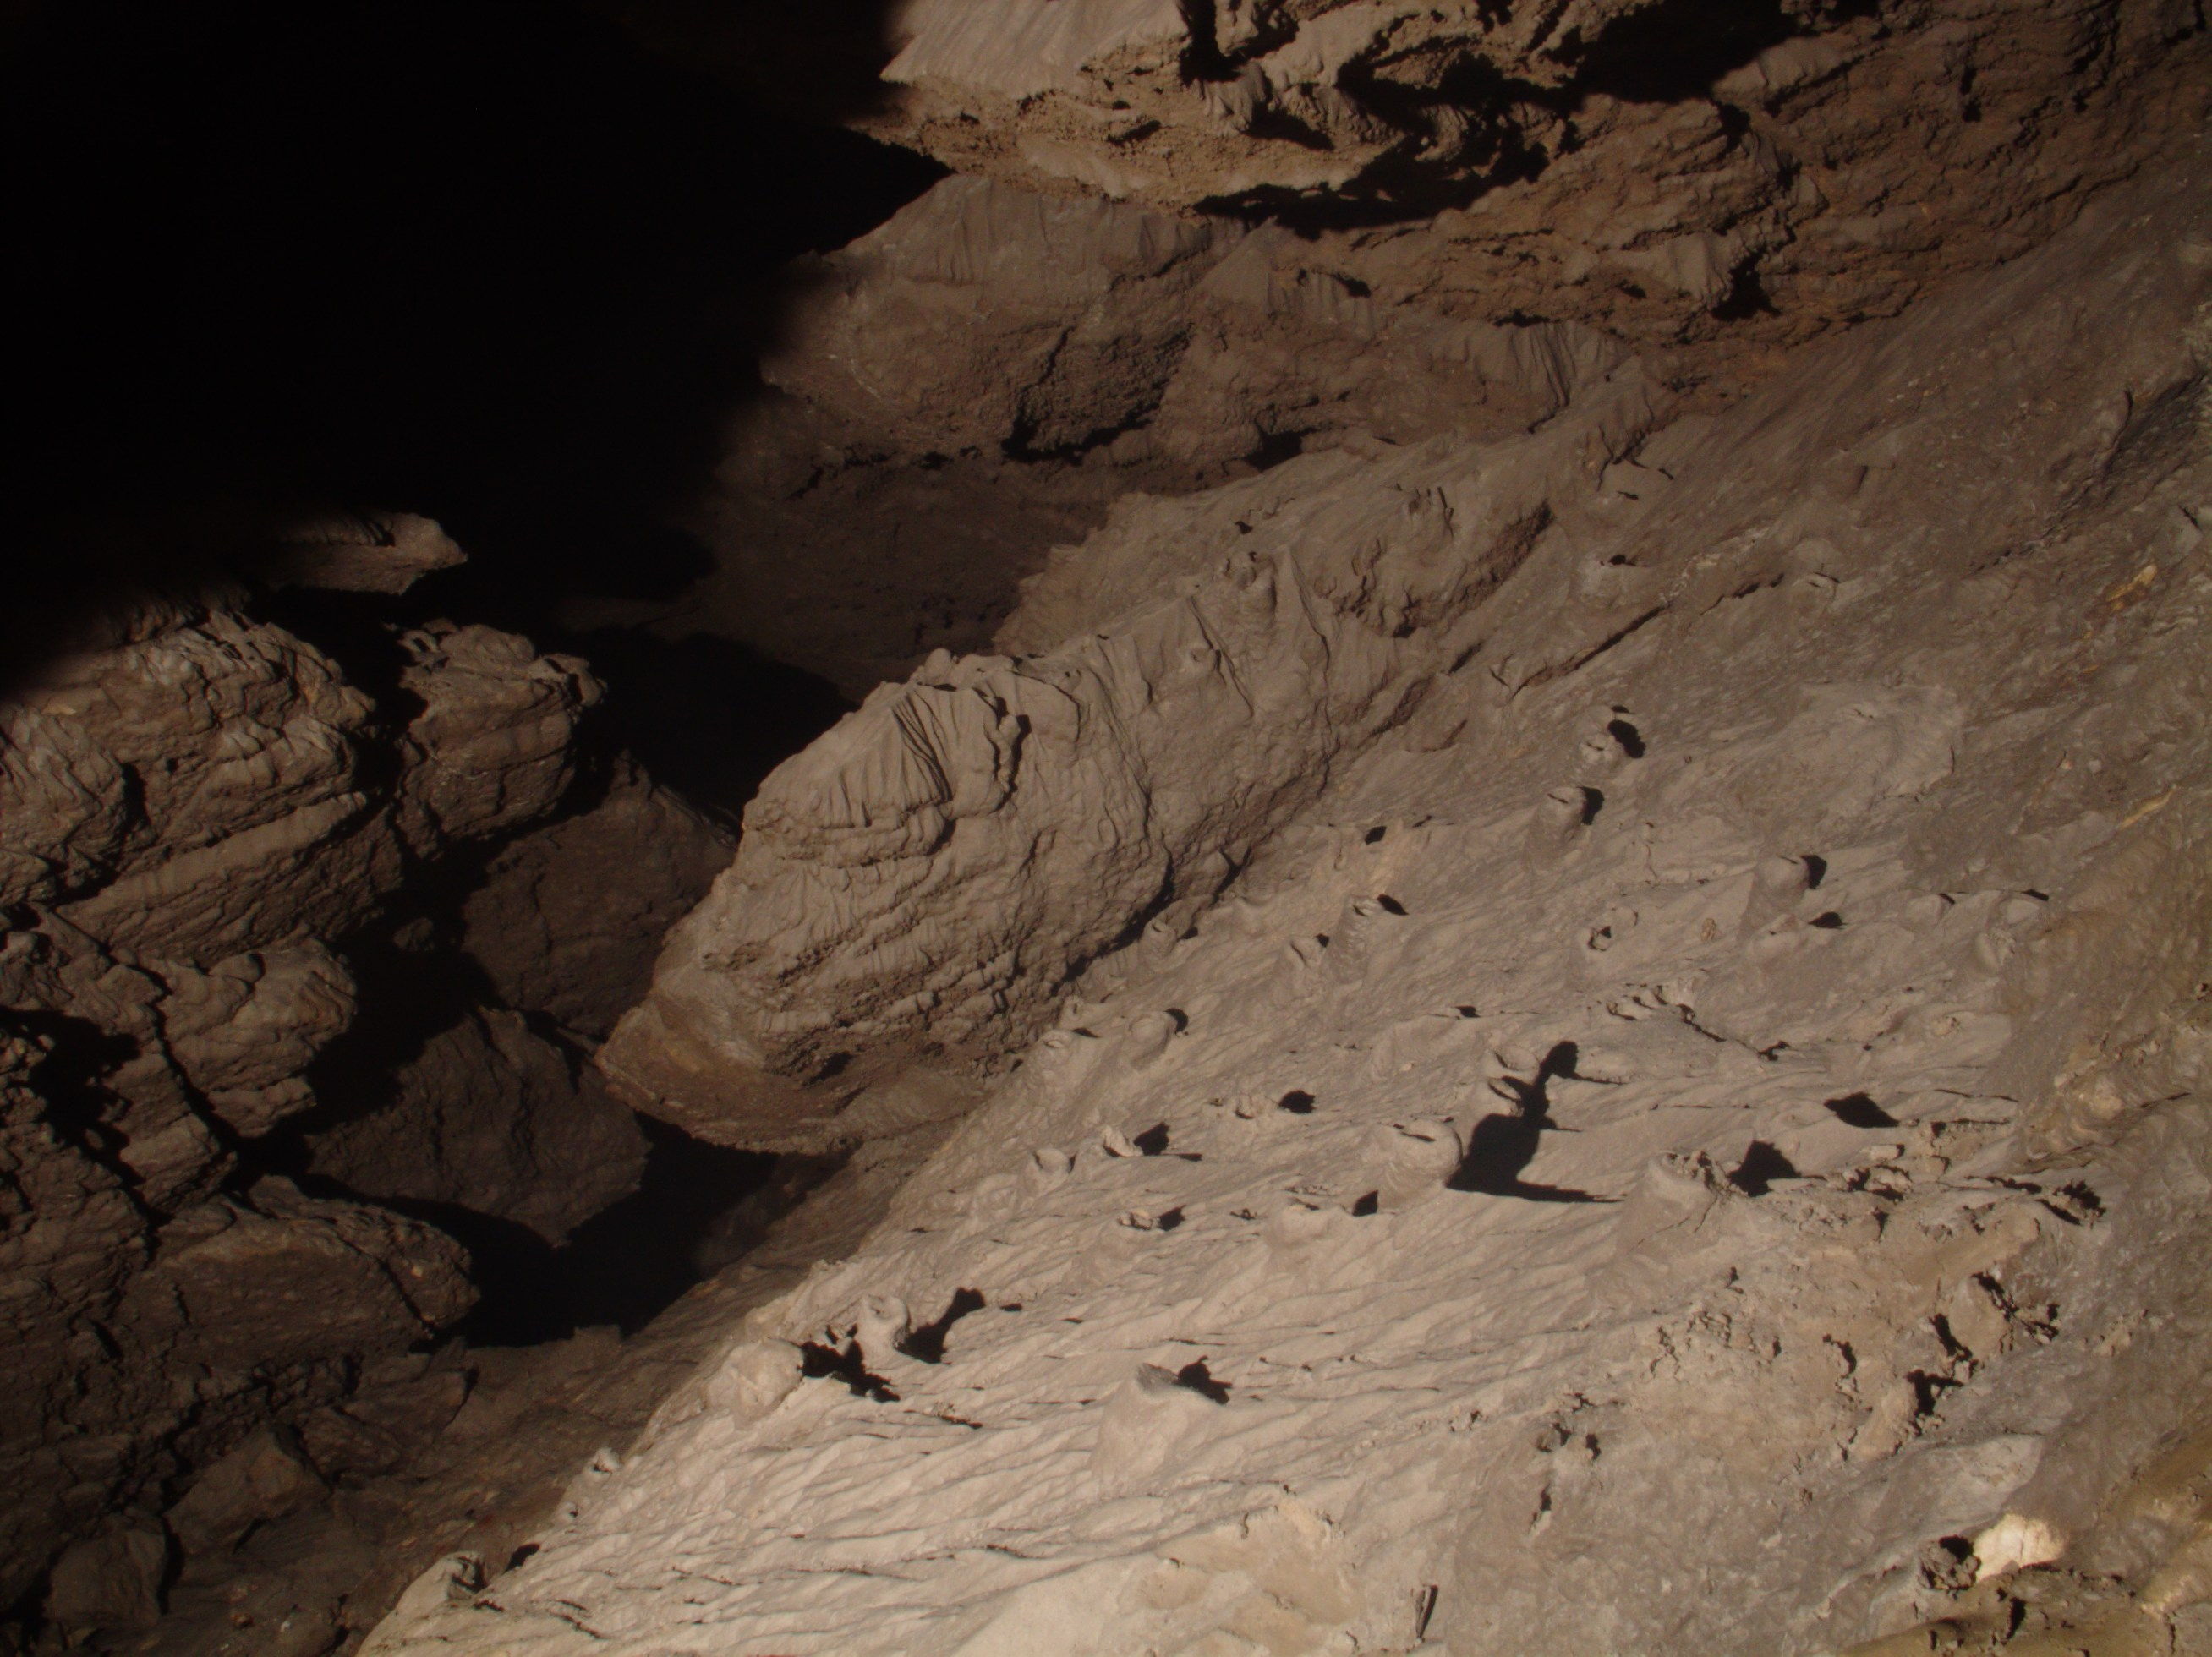
\includegraphics[width = \textwidth]{2011/winter_journey/2011-08-05-03.13.20-Jarvist Frost-CanonG5-CRW_0127 - Silt deposits in Chamber just before bottom Winters Journey--orig.jpg}
\caption{Silt deposits in the passage \passage{Winter Journey}. \pic{Jarvist Frost}} \label{silt winter}
\end{pagefigure}

I pack the gear away, and quickly return to the others, with one last
look back from the massive muddy boulder into this sad chamber, and
listen briefly to the tantalising noise of tumbling water.

Now begins the real efforts of our trip. It's 350 m vertically back to
Camp \passage{X-Ray}, but the distance and height really doesn't matter.
This is a fight against tiredness.

We eat the last of our bread, split the equipment, and head out. At the
beautiful cascade pitch that demarcates \passage{Dream1} and \passage{Dream2}, we stop on
the ledge and make use of the massive Sigg bottle of meths, tuna can
stove and mess tin. We have no provisions, but the hot water is lovely
itself.

Jim is so cold without thermals and in his Warmbac that he gets into his
survival bag at every stop, pulling it down from the top like a massive
condom. I fold myself into a crack in the rock, resting against my
boots, kneepads and helmets so that nothing touches the freezing rock.
My eyes close, listening to the water falling down the pitch, that odd
sensation of sinking into the Earth as sleep snatches your
consciousness. My eyes open as I shiver, \bignote{Jim is Penis-in-bottle again,
his condensation filled survival bag lit from within, like some terrible
angel}.

Andrej wakes up and suggests we move on. Wearily we do. At the end of
\passage{Dream}, where the squeeze onto the pitch is, Jim has a desperate urge for
a shit, and has just taken off his harness to get through the horizontal
pitch head squeeze. ``Oh God, wait until I'm up!'', I plead as the
column of water thunders past. I make it to the rebelay ledge as the
chicken nuggets go flying over my shoulder.

Andrej ahead, I go up \passage{Insomnia}. It could really do with a
deviation, but with one hand spare you can hold onto flakes on the wall
and do it yourself. I call rope free to Jim, and get a response. At the
traverse I wait, clipped in. I fall asleep, and wake an indeterminate
time later, and bellow to Jim. I think I wake him up as well, as soon
the rope starts twitching as he comes up.

\passage{Republika} is really quite wet on its natural hangs. Back at \passage{Red
Cow}, we have a brief rest. Already, we seem so much closer to home.
Whereas below here, you are at the mercy of the weather and the water,
this massive phreatic is a warm friendly place. It is certainly a
fantastic base, psychologically, practically and logistically for a camp
to explore the deep area.

The main hazards overcome (and the risk of flooding) we carefully pick
our way back to Camp \passage{X-Ray}. Above the hidden pitch in \passage{Leprechaun},
we have another snooze. \bignote{Awoken by a dream, I check my oversuit pocket --
bonanza, just like in the dream, a chocolate bar!} One bite each and it's
a massive difference, but the very last we have. We are but machinery.

Onwards we go, just keep moving, slowly, so slowly. The climbs seem so
difficult now, limbs so uncoordinated, brain so slow in seeing hand
holds and thinking things through. Back at \passage{Big Rock Candy
Mountain}. I check that Jim is happy to head back to camp himself, and
head up, head home. Nice and warm now at least, I thread my way along
\passage{Friendship Gallery} and, eventually, so back to camp.

Hot tea, supper, warm fleece to wear and a beckoning bed. Jim does not
appear, eventually a rather more refreshed Tetley is dispatched to find
him, locating him staring down \passage{Prima Junction} wondering if that's where
he came from.

Tetley and Clare, now that Gergely, Izi, Jana, and to a lesser extent
Dan and I have all put in the bolts to conquer \passage{Stuck in Paradise},
head off to go and push the draughting crawlway at the bottom. This area
sounds like a fantastic lead, and absolutely amazing that all this
passage grew from a ludicrous find on a bouldery ledge halfway down a
pitch.

\margininbox{6/8/2011 9am}{\passage{Let na Drugi Svet} -- \passage{Krtkova Dobra Dela} -- \passage{Heroj
Telemarka}\ldots{} \ldots{}BAM! Samo fell, so we're going out now. He had
``luck'' that he fell in water. There are 3 leads with water way, 2 up
\& 1 down. \name{Karin}}{\logbook}

Marzipan and Sleep. I'm awoken by noise, quietly spoken Slovene and the
rustling of tinfoil. I awake again. The roar of the gas stove. It must
be much later, but the song is the same again, the stereo is playing
Blondie on loop. Nothing makes sense, my head too woolly to understand,
to wake up enough to comprehend.

Eventually Andrej wakes up properly and speaks to the disembodied
voices. It's Samo, who's taken a nasty fall and split his knee. He's
come to camp with Karin. They're cold, sitting on the edge of the tent
in damp caving gear, wrapped in rustling survival bags.

A misunderstanding, \bignote{in being concerned to let us sleep they were keeping
us awake and torturing themselves}! Andrej sorts them warm clothes, and
frees his bed for the two. Instantly back to deep sleep. Andrej gets
cold and crawls in between Jim and Samo, wrapped in all the spare
fleece. I find myself pressed immobile between the tent and Jim's
reassuring bulk, and hold this awareness for a second or two before I
drop into deep sleep once more.

\name{Jarvist Moore Frost}


\section{Finding Salvation}


\margininbox{Salvation}{
     \begin{itemize}
    \item James "Tetley" Hooper
    \item Clare Tan
    \end{itemize}}{\explo}

Following our 16.5 hour push to the bottom of \passage{Vrtnarija} the
previous day, Tetley and I without discussion agreed on a pleasant
`bimble' for our last push of the expedition. Surprised that none of the
other teams had pushed Gergely and Izi's lead below \passage{Stuck in
Paradise} yet, we seized the opportunity with both hands: roll on
glorious horizontal passage!

We made our way to the pushing front leisurely, scrounging for hangers
and maillons along the way after realising at \passage{Cheetah} that we'd
forgot to pack any, and enjoying a civilised ginger cake (``It tastes
better sliced!'') and ciggie break in \passage{The Throne Room}.

Finally we got to \passage{Stuck in Paradise}, the muddy pitch from hell
and the furthest either of us had been in this part of the cave.

``After you,'' grinned Tetley. ``Good luck.''

I climbed a short rope to gain a traverse and the start of the descent
proper. We had heard the horror stories from Gergely, Izi and Jana, but
this is one pitch that has to be experienced to be believed. Sticky mud
coated everything---maillons, knots, cowstails---into blobs of uniform
brown. Globules of wet mud oozed down the pitch walls of their own
accord, punctuating our descent with timely `plop!'s. Later, on our
return, our jammers would slip back down without biting, so thick and
slippery was the coating of mud on the rope. I let out an incredulous
chuckle.

``How is it?'' came a shout from above.

``It's okay, but don't C-rig!'' I warned.

God knows how long it was before we finally reached the bottom, very
relieved, 18 bolts and 70 metres later. All respect to Dan, Jarv, Jana,
Izi and Gergely especially for bolting and rigging the pitch, it was a
hell of an effort and superbly done: most beautiful rigging in most
squalid conditions!

A couple of fags for Tetley and it was time to rock and roll. 150 metres
of painful crawling over uneven rock---\passage{Penitence} passage, as it
was aptly named. We stopped for a bit to admire the clean, white
stalagmites midway through, but our minds were firmly on getting to the
boulder choke at the pushing front. Thankfully we reached it soon
enough, moving the tacklesack through the passage was starting to get
tedious.

We set about digging through the choke, spurred on by the strong draught
on our faces. After a while of shifting rock and wanton destruction with
the bolting hammer, we broke through to delightful walking passage. Ahh
yeah! We shook hands and raced down the passage. It soon degenerated to
a crawl, but just as I rounded the corner it opened up once more, this
time yielding delicious, milky sand.

``Game on!'' shouted Tetley, and I am sure the massive grin on his face
was mirrored on mine.

``Before this gets trashed, take 10 steps and look back,'' he said.

\margininbox{Dig for Victory}{

\textit{6/8/2011 4:20 a.m.} -- Firstly, respect to those, especially Gergely, who pushed \passage{Stuck in
Paradise}. Amazing push\ldots{} truly heroic etc. Praise to to the
electric drill!

Clare and I went down to push the extensions beneath. We dug through the
boulder choke at the end of \passage{Penitence} to find \passage{Salvation} -- 200 m
of mostly walking horizontal passage. Drafting lead left. Forgot to take
water, despite my own `top tip' early this expo, hence pretty dehydrated
after 10 hrs caving, no water to be found. Grade 1 survey to follow
after sleep. A great day, only marred by news of Samo's injury, I hope
he's OK. \name{Tetley}}{\logbook}

I did as suggested, and the sight of my lone pair of footprints in
otherwise unblemished sand looking back at me sparked a strange tingling
in the pit of my belly. I'd heard and read such tales about the magic of
exploration before, of course, but I'd always treated it with a degree
of scepticism, if not actually dismissed it as outright hyperbole. But
now, confronted by such an experience myself, it felt intangibly
special.

``Shall we call this \passage{Salvation}?''

``Funny\ldots{} I was just thinking the same myself,'' I replied.

Euphorically, we whooped down the passage, wordlessly agreeing to
exchange leads every so often. When we finally stopped at a junction for
a chocolate break, Tetley started giggling, ``Clare, we're such tarts!''
I couldn't believe my good luck, not only on this trip, but also on the
whole expedition---not in my wildest dreams had I imagined enjoying
myself as much as I did on the mountain or finding so much passage
underground. On one of our previous pushing trips, Tetley, three-parts
silly and one-part sage, told me, ``This mountain is really strange\ldots{} 
sooner or later, \passage{Mig} always rewards those who have put in the effort.'' I don't know about effort, but this was one hell of a reward\ldots{}

In all we found about 200 m of passage before time signalled the end of
our discoveries for the day, and we left an easy squeeze with a howling
draught for next year's team to push. Less exciting but nonetheless
worth a quick look was a sandy dig off to the right of the junction,
reminiscent of the digs below \passage{Big Rock Candy Mountain}.

Battling dehydration, we raced our callout back to Camp \passage{X-Ray}.
The return journey was smooth apart from -- big surprise -- \passage{Stuck in
Paradise}. There are sections of this pitch that are quite loose, so we
agreed to ascend the pitch one at a time. Unfortunately, we neglected to
take into consideration 1) the fact that the pitch is actually made up
of a series of chambers and 2) the noise-absorbing qualities of mud.
Which led to a rather comedic (though it didn't seem so at the time!)
situation:

``IS THE ROPE FREE??'' I'd shout.

``ROPE\ldots{} FREEE!'' \bignote{Tetley was shouting as loud as he could from
above as well, but I heard nothing}.

``IS\ldots{} THE\ldots{} ROPE\ldots{} FREEE?'' And so on.

This went on for a good 15 minutes at least. Eventually I thought, fuck
it, he must be at the top by now, I'll just go up. Ascending the pitch
was a rather harrowing experience and I arrived at the top to find a
rather cold Tetley and a half eaten tin of fish. Yet I knew that for the
next 11 months I'd be dreaming about returning to this part of the cave.
Oh, the lure of deep cave exploration\ldots{}

\name{Clare Tan}



\section{Drink Your Own}

Fratnik departs with Karin \& a taped up Samo in our night. After a
delightful lie in, Jim and I slowly get ready for caving, taking the
opportunity to absorb hot calories from the stove and round after round
of drinks. Wet wet wool socks. Jim is horrifically stiff, he's barely
done any SRT in the last 7 years! We head off for \passage{Serpentine}.
It's Jim's first passage down \passage{Leopard} and brief sight of the
formations. I lug my photo gear along, and Jim indulges me as I try and
record the formations in the \passage{Longwater}, and take a couple of mineral
samples and a piece of broken straw.


\begin{marginfigure}
\checkoddpage \ifoddpage \forcerectofloat \else \forceversofloat \fi
\centering
 \frame{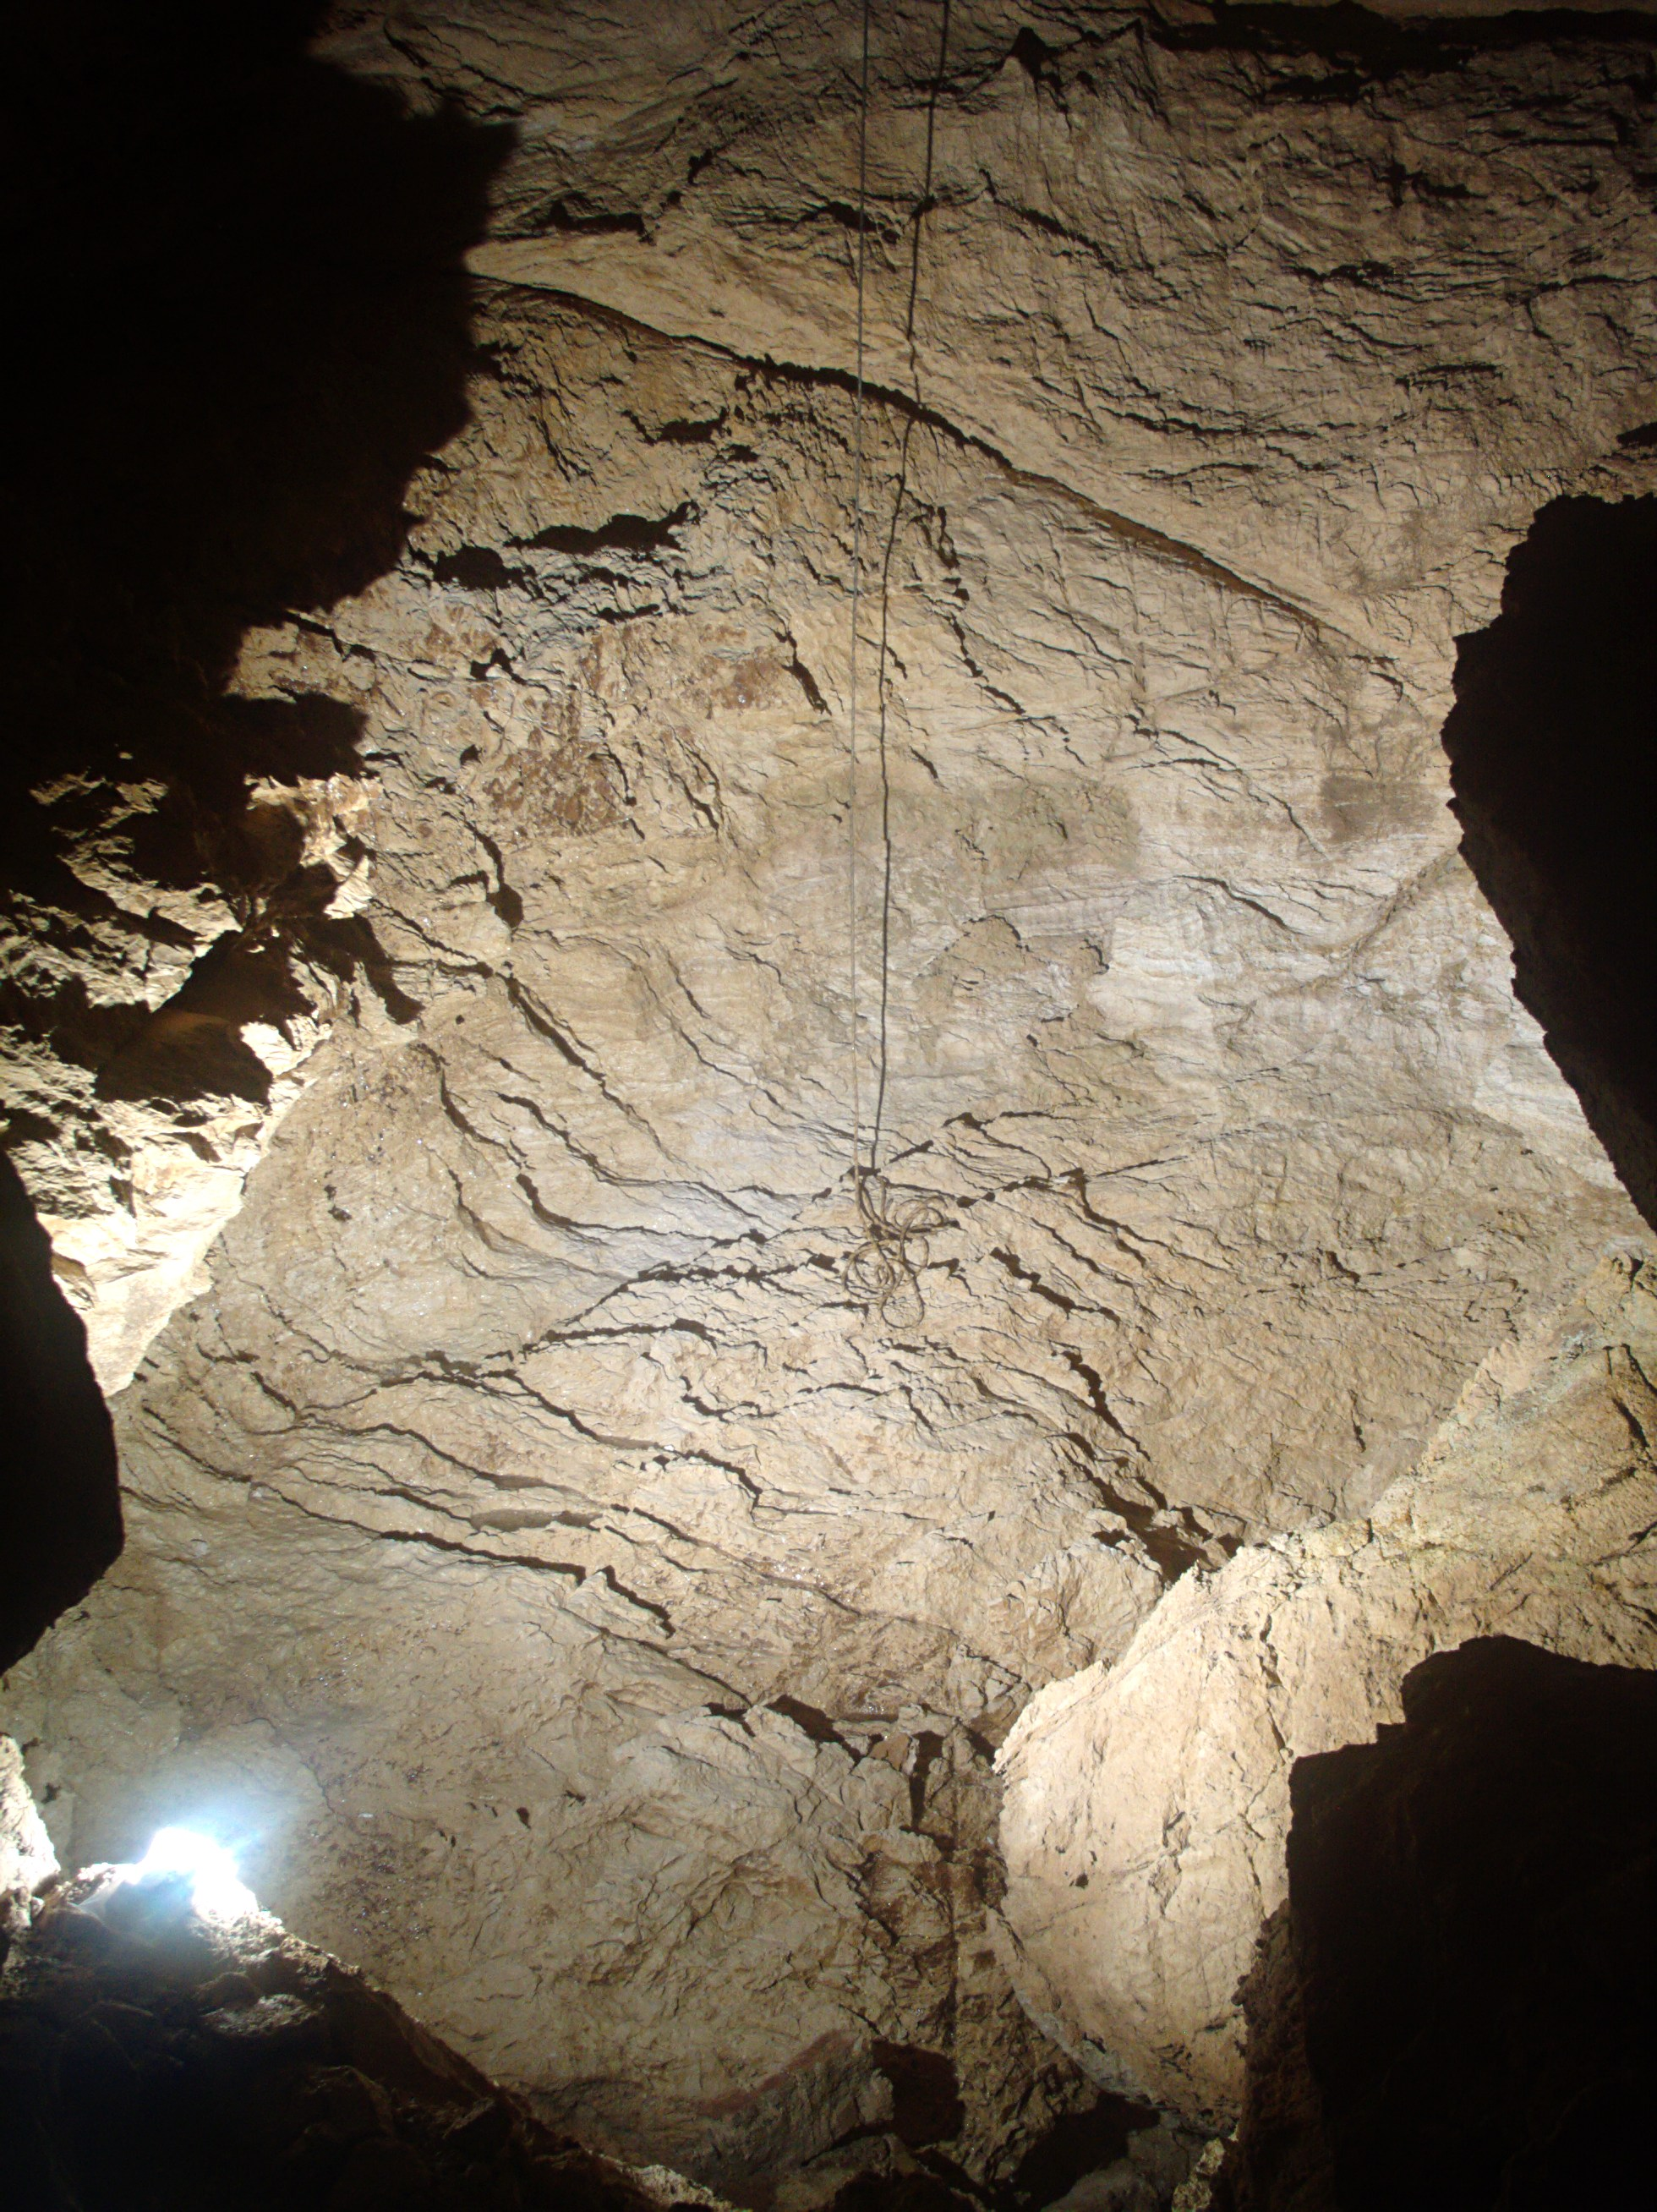
\includegraphics[width=\linewidth]{2011/winter_journey/2011-08-06-05.04.38-Jarvist Frost-CanonG5-CRW_0161 - longwater pitch--orig.jpg}} 
 \caption{\passage{Longwater} pitch. \pic{Jarvist Frost}}
 \label{longwater}
\end{marginfigure}


Back at the end of \passage{Rotten Row}, the pitch doesn't look hopeful. If
anything, it is wetter than every previous time I've been here.

Having just been to \passage{Republika}, I can't help but try and interpret
what I see in terms of it being the same passage. Dangling from the end
of Dan's bolt traverse in the ceiling of the rift, I can look down into
a chamber, large boulders and bedrock with the two streams crashing down
in different locations. God, if only we'd had the sense to put some
retro-reflector markings or something down there! Then we'd know for
sure. Was I walking along there less than a day ago?

Jim is stiff and cold, and so rests in his survival bag in the quiet,
dry, side chamber. I have no drill, and I'm not super hopeful in getting
down. I rejig the rigging, turning a hastily placed drilled deviation
into a rebelay and then attempt to rig a natural deviation to further
swing along the rift and pass over the top of the inlets. Again and
again it falls off, eventually I give up.

With a drill and sufficient bolts, you could just keep on going in the
rift and reach the far, dry side. But no such luxury now. Spider-walking
along the left wall, I reach the ``\passage{Duffers Drop}'' inlet and confirm
that I can see the bolt in the floor. It might actually require fewer
bolts to successfully rig from here.

\margininbox{Drink Your Own}{
     \begin{itemize}
    \item Jim Evans
    \item Jarvist Frost
    \end{itemize}}{\explo}

The far side of this (left wall) inlet, I abseil down to a nodule of
rock at the start of the dry bit of this rift, could I rig a rebelay?
I'm getting wet now, ricocheting splashes from both inlets landing on
me. The sling slips, again and again. I try a deviation. It falls off.
This is hopeless.

Defeated, I'm left dangling from my skyhook equipped cowstail and wonder
what I should do. Nowt but to survey I guess. I tie a bunch of maillons
to the end of the tape, and lower it down into the chamber below. It
lands on a boulder, but gives me a reliable distance (15.10 m). How
hilarious it would have been to have someone in \passage{Republika} at that
point, watching this fistful of metalwork being lowered from the Gods!

Retreat! Back up the rope and do my best to survey. Jim is looking
utterly miserable, tired and cold.

\margininbox{6/8/2011 1:20 pm}{

Another camping trip drawing to a close, quite probably my last pushing
trip of the expo! Just waiting for Jarv and Jim to return before we
start our bid for the surface. \name{Clare}}{\logbook}

We've a lot to do on the way back to camp, but there's no thinking
involved so we just quietly get on with it. The bolting kit, pushing
rope and photo kit all need to be returned, and we intend to derig the
whole of \passage{Serpentine}. To this end we have taken one of the massive
tackle sacks (used to transport the sleeping bags down) from camp. Back
at \passage{Longwater} we already have two filled normal tackle bags, and
start feeding rope into the monster.

It is a struggle up ``\passage{It Will Rain}''. I wonder about its height,
and whether it was miss-surveyed due to the Laser rangefinder catching
the wall. Certainly it seems to have a hell of a lot of rope for a `35
m' pitch.

Massive bag stuffed with rope, I can barely prussic. Jim has led on out
with the two normal sacks. Amazingly, he's waiting for me at the top of
the pitch! Together we move the tackle bags along \passage{Serpentine}. It
is tough work, taking both of our strengths to wrestle the monster
through some bits.




	\begin{figure*}[t]
	\checkoddpage \ifoddpage \forcerectofloat \else \forceversofloat \fi
		\centering
		\begin{subfigure}[t]{0.49\textwidth}
			\centering
			\frame{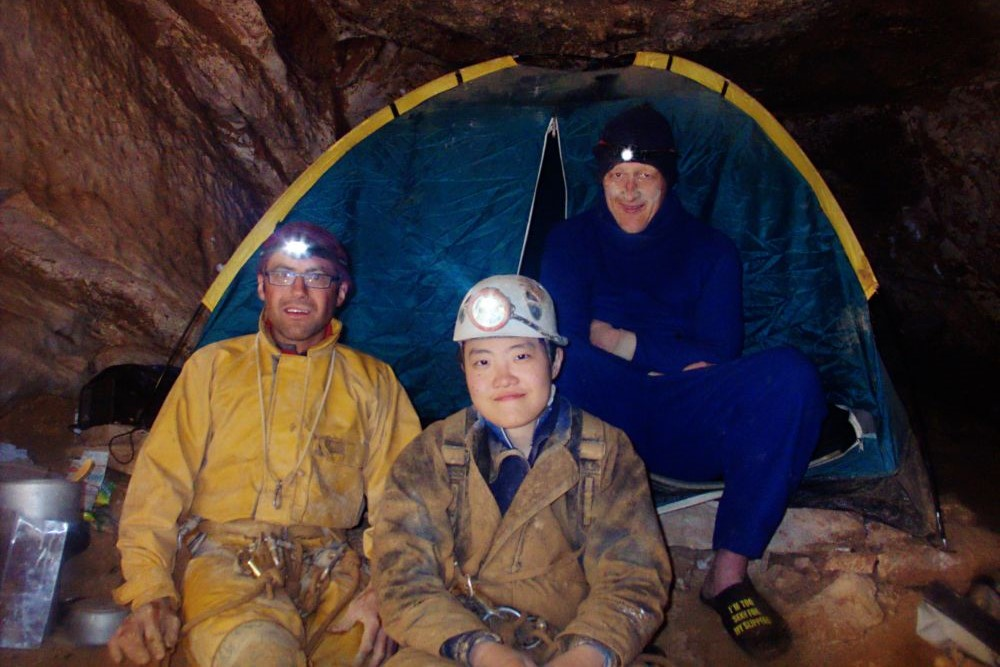
\includegraphics[width=\linewidth]{2011/winter_journey/2011-08-06-13.40.56-Jarvist Frost-CanonG5-CRW_0166 - jim tetley and clare at camp x-ray--orig.jpg}}
			\caption{13:40.56}
			\label{jim tet clare xray}
		\end{subfigure}
	\hfill
		\begin{subfigure}[t]{0.49\textwidth}
			\centering
			\frame{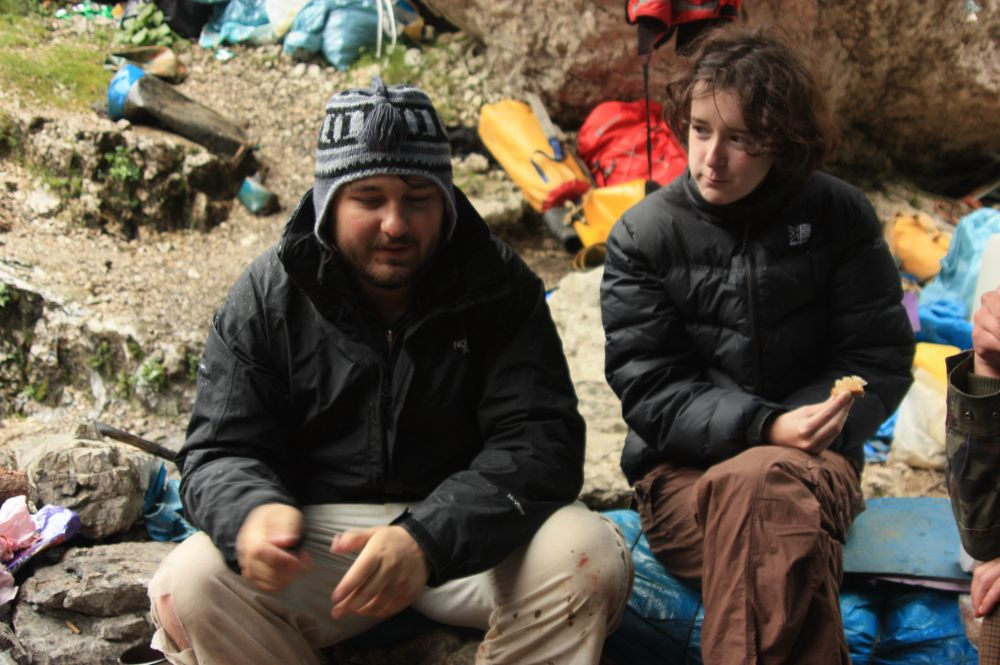
\includegraphics[width=\linewidth]{2011/winter_journey/2011-08-06-13.41.54-Gergely Ambrus-Canon450D-IMG_1012-Wet Cold Bivi--orig.jpg}}
			\caption{13:41.54}\label{alex nia bivi}
		\end{subfigure}
		\caption{Though these two photographs were taken less than a minute and a kilometre apart, they show two different worlds.
  \textit{(a)} Tetley, Clare and Jim at underground camp. \pic{Jarvist Frost}
  \textit{(b)} Alex and Nia wrapped up warmly in the \passage{bivi} on a wet and cold day. \pic{Gergely Ambrus}}
	\end{figure*}



Back at The \passage{Albert Hall}, we continue along the passage with our
treasure. Jim moves forwards with the massive bag, I have the two more
manageable ones.

Back at camp, we wake Eric and Tjaša, and soon find ourselves ensconced
in the sleeping bags and drifting off to sleep once more.

Eric and Tjaša come back early from their pushing, having decided to just survey and then come back as the \passage{Let na Drugi Svet} cascades were getting unpleasantly wet. With little chance of pleasant pushing, Jim and I decide to pack up and head out. Everything is fine till we get to \passage{Alchemy}, when I realise we can hear the water tumbling down \passage{Space Odyssey}. The cave is going into flood!

\passage{Swing} is actually OK, if you self deviate. Similarly, \passage{Tera} and \passage{Nova}, though now terrifyingly noisy places (the water was splashing up to about 80-90\% of the clean rock), were dry hangs.

\passage{Pico} was something else entirely. There was heavy rain falling over the
entire bottom of the pitch. Near the \passage{Tera} entrance, there was a sheet of
water falling, and perhaps most disturbingly, a stream is cascading down
the rockface of \passage{Pico} itself, intermingled with the rope on the last few
rebelays.

Jim gave me a shout from near the top, and I dashed across the chamber
avoiding the heavy water and sprinted up the rope. The scalloped ledge
you pass on the left at about +25 m was collecting a waterfall that came
through a hole right up in in the high ceiling and directing it down the
lower hangs. It was pretty bad. By the time you got to the \passage{Captain
Kangaroo} branch, you were out of the worst of it, and just had to
contend with a few drips.

\passage{Piston} was similarly drenching, the stream coming over the lip so
quickly that it bounced off the far wall and splattered down over the
hang. Nearer the deviation, it was fine.

\margininbox{7-8-11 13:00}{

A very long sleep but worth it. Jim is feeling a lot less stiff \& my
back is popping less. Certainly the derig yesterday exacted its toll.

Camp is looking rather bare, nil shitbags, meths, sugar, hot choc, rice.
The train is crashing \& it's time to get off. \name{Jarv}}{\logbook}

The others in the \passage{Urinal Series} were splashy, but not as bad. \passage{Laurel}
itself was wet for sure, but more in a sort of `soft rain' way that
didn't feel anywhere near as threatening.

The last few pitches were a definite struggle for Jim, so stiff he was
just getting a few 10s of cm of height with each prussic step.

Back on the surface once more, a slow walk back to the \passage{Bivi} over a wet,
slippery, plateau for some food and needed rest.

This was a sleep deprived and rather unnecessarily sufferable trip, but
nonetheless through grit \& teamwork much was done, the deepest point
since 1998 was explored to on \passage{Migovec}, photos were taken of the deepest
point of an Alpine cave, all leads were surveyed and the entirety of
\passage{Serpentine} was derigged to free rope, hangers and maillons for
exploration in future years. Not only did we have our Penguin's Egg, but
we had brought it all back home.

\name{Jarvist Moore Frost}


\newpage

\begin{figure*}[t!]
\checkoddpage \ifoddpage \forcerectofloat \else \forceversofloat \fi
    \centering
        \frame{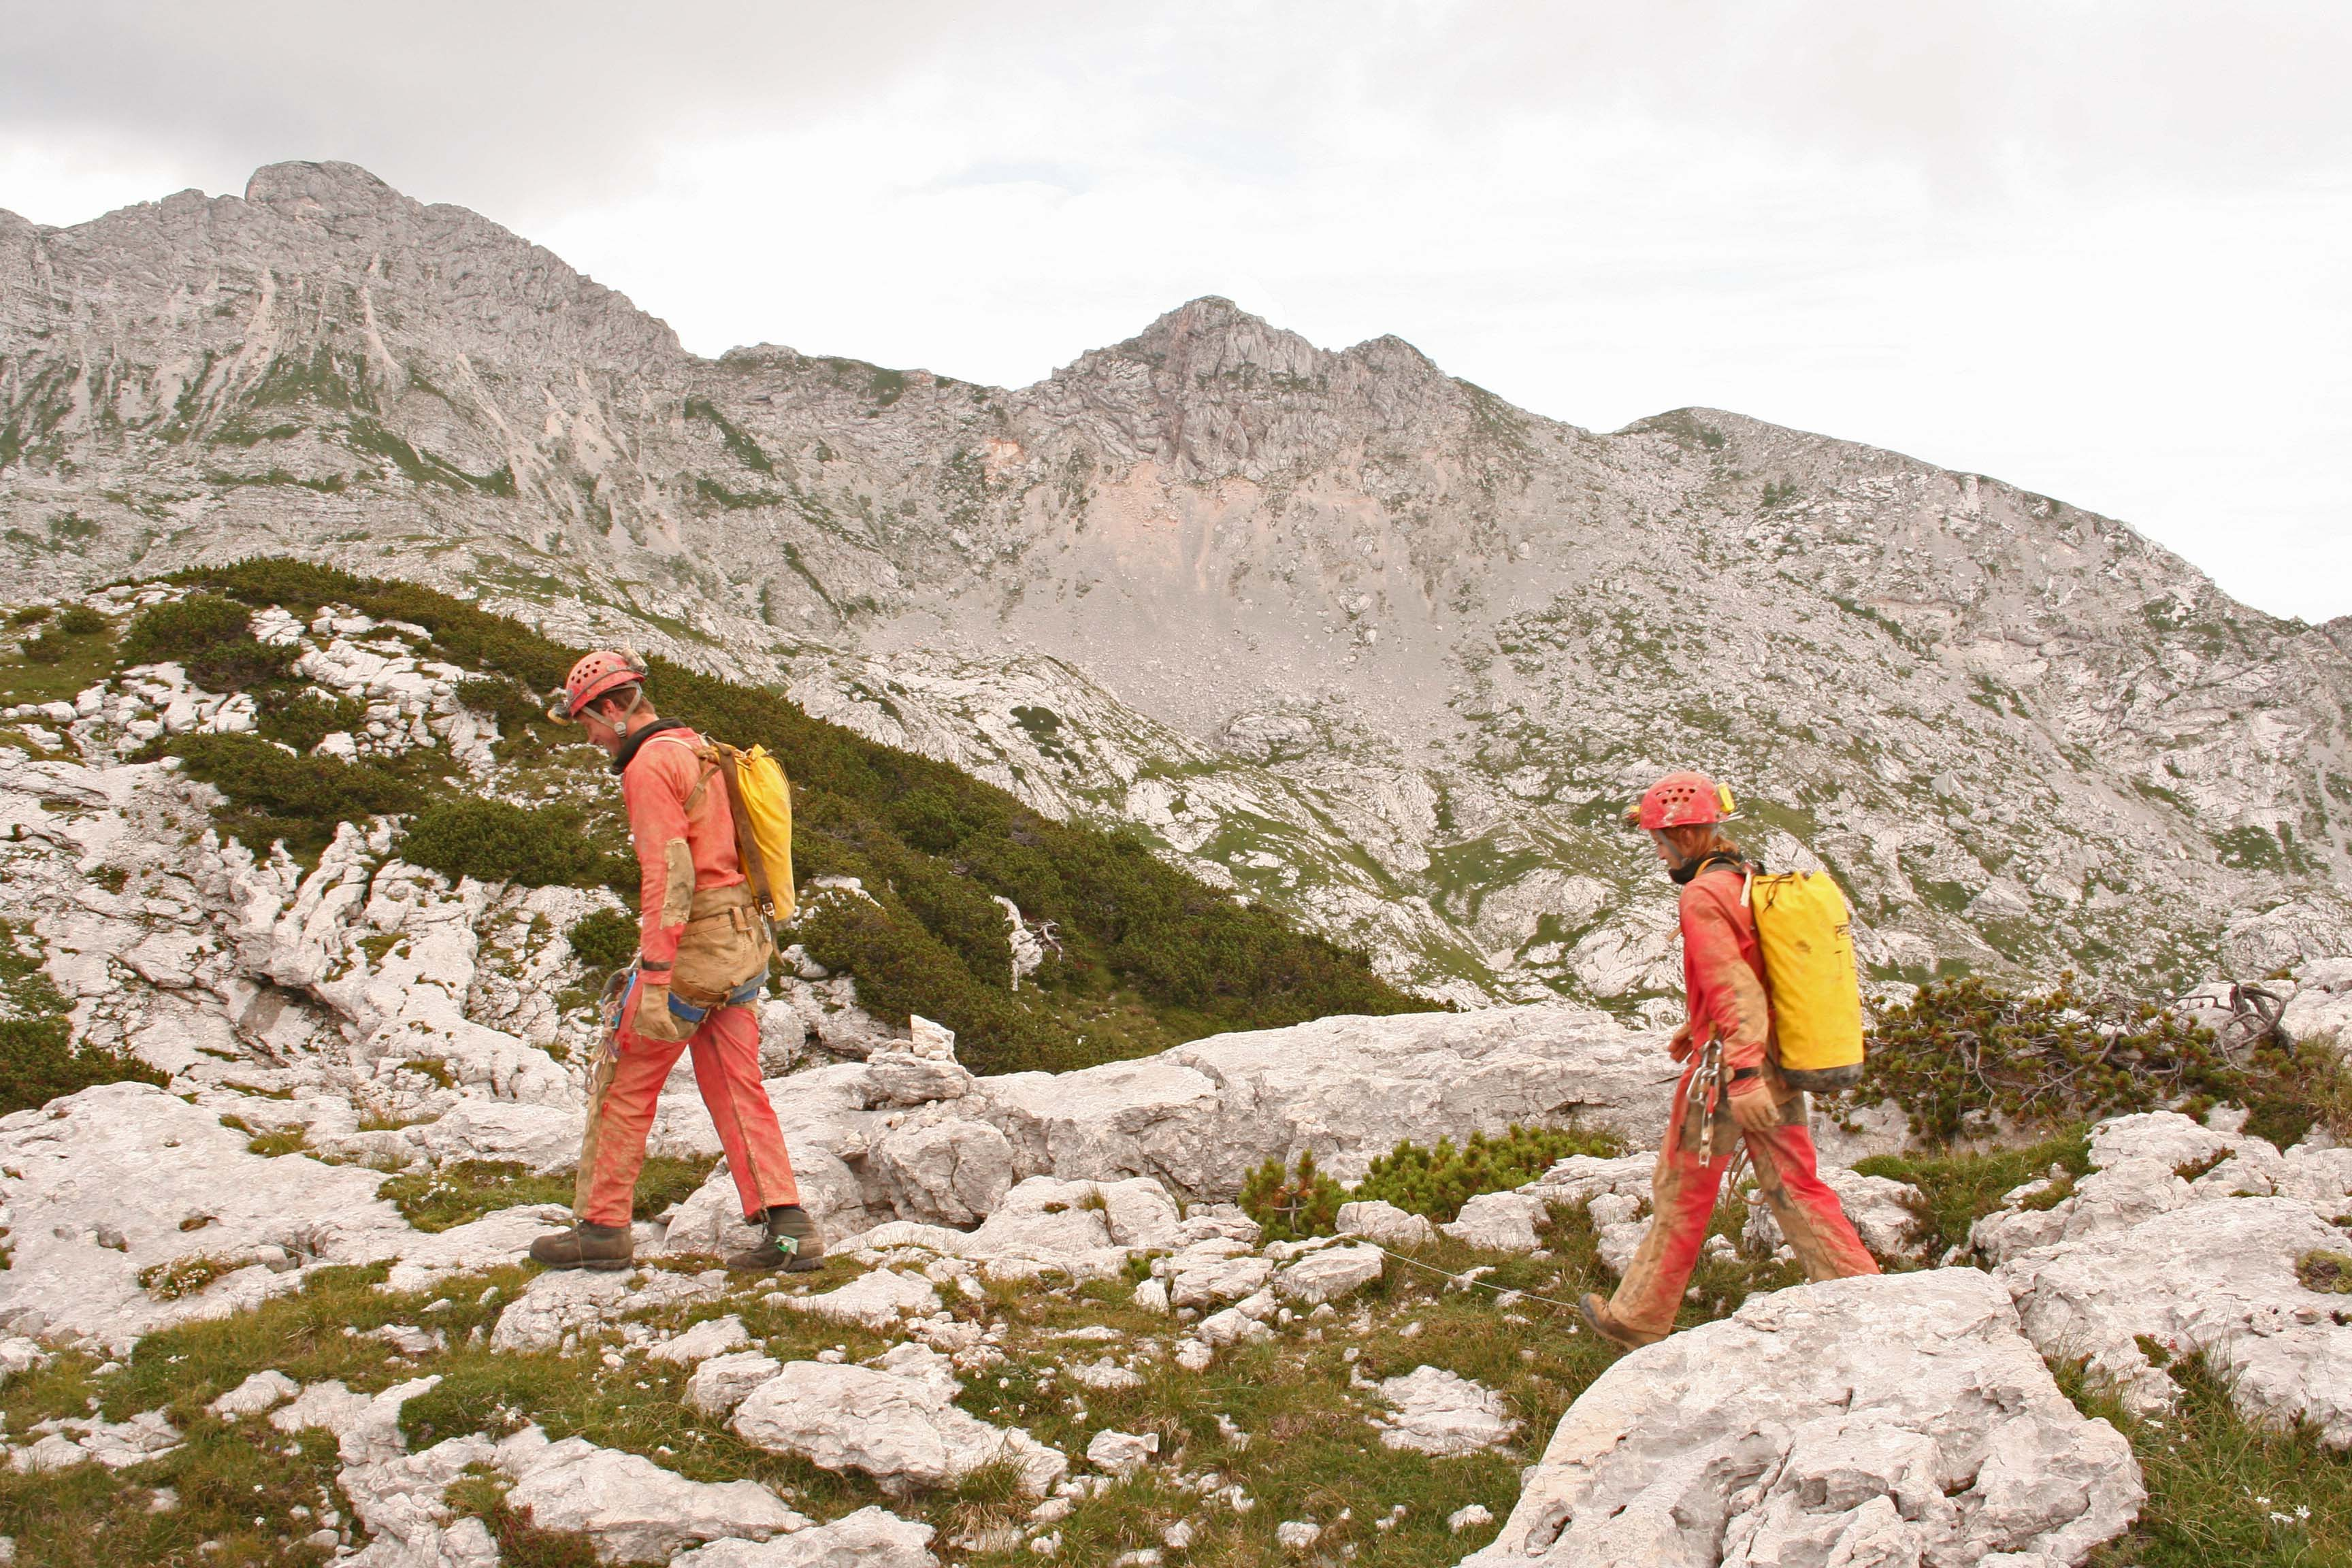
\includegraphics[width=\linewidth]{2011/winter_journey/2011-08-05-10.37.03-Jana Carga-Canon 350D--orig.jpg}} 
        \caption{Heading to the caves with a striking ridgeline behind. \pic{Jana Čarga}} \label{plateau tjasa}
\end{figure*}

\section{Undergound logbook: Heroj Telemarka and the end of 2011's pushing}

\textbf{7.8.2011: 1700}

We were surveying and get very wet. We had surved[sic]\sidenote{where 'surved', read 'surveyed' or 'survey'} \passage{Heroj Telemarka} that
found Samo \& Karin yesterday. Samo falls into the water and there is
also our surveying stopped. That is on the left side (part on Karin's
drawing where are ``two amazing lakes''). Then we went to the right.
Karin had written that there are 2 meanders but is only one. It just
looks like there are 2 because they're one above another but after a few
metres they become one. That meander ends after 30 meters. There is
water so we couldn't get over it. I think it is possible but you get all
wet. So we end after 30 meters. We do the last station on a rock which
looks like this but we didn't put any paper because it hangs from the
cealing (strop -- SLO).

{[}Tjaša's sketch referred to above{]}

We decided that the name will be the same as Karin \& Samo gave it to
the nearer part and because they told us to go there. So, it's named
\passage{Heroj Telemarka}.

We eat 2 frutabelas there and go surveying the part which founded I and
Grega few days ago (that little canyon). We named it \passage{Krtek in Orel}\sidenote{\textbf{Mole and Eagle}}. The
last station is above the bigger pitch. We didn't surved it down because
we didn't want to get wet. Anyway, when we went back + swing on a rope
accidentally under the waterfall and get wet. And Erik get wet in the
squeeze in \passage{Krtkova Dobra Dela}. So, we were all wet in the end.

Shit happens : )

Under the bigger pitch Erik bolted something and it's possible to go
down. If you follow the water you come to a lake and it's impossible to
get there without getting wet (the level of the water is high to knees,
something like that). The possible way going further is above the water.
It's something like passive meander, it needs to be looked one more time
to see if it's possible go further without going into lake.

We're going out today. See you and good luck to everybody!

\name{Tjaša Rutar}


\tweet{1:08PM Aug 8, 2011}{VRTNARIJA 10810m long, 888m deep!Heavy rain,early end to pushing.Deepest point 10cm rift w loud sound of stream.Big phreas extends to E}


\textbf{7.8.2011: 2100}

Erik and Tjaša. As it seems we are staying in camp because there is a
waterfall in \passage{Zimmer}. So, good night.

\name{Tjaša Rutar}

\textbf{8.8.2011: 1100}

The water calms down slowly but there is still a lot of it in \passage{Zimmer}. We
hope that on the surface cavers don't panic because we won't come out at
the callout.

Today is Erik's mother Maria birthday. It seems that \bignote{he will miss the party}.

\name{Tjaša Rutar}

\textbf{8.8.2011: 1400}

Much more water than in the morning.

\name{Tjaša Rutar}

\textbf{9.8.2011: 1400} 

Finaly! Gergely and Tetly come in camp. It means we can go out.

Thanks for nice \& warm camp! Tjaša \& Erik.

\name{Tjaša Rutar}

\textbf{9 Aug 2011: 13:45}

This tear the last time in Camp \passage{X-Ray}! We wanted to come down
with Karin to push \passage{Salvation}, but the storm put us off. So today we came
in 1.5 hours with Tetley to check if Tjaša and Erik were good, after 24
hours their callout. Luckily, everything is all right and the camp is
rocking with music! Great times! The cave is still wet but \bignote{it is time to
go}. Another year, another expo, another success. See you next year!

To the connection and the new passages and to infinity.

\name{Gergely Ambrus}

